\documentclass{classrep}
\usepackage[utf8]{inputenc}
\usepackage{color}
\usepackage[utf8]{inputenc}
\usepackage{amssymb}
\usepackage{polski}
\usepackage[polish]{babel}
\usepackage{amsmath}
\usepackage{amsfonts}
\usepackage{lastpage}
\usepackage{fontawesome}
\usepackage{graphicx}
\usepackage{float}
\usepackage{geometry}
\usepackage{caption}
\usepackage{subcaption}
\captionsetup{compatibility=false}

\DeclareUnicodeCharacter{00A0}{~}

\studycycle{Informatyka, studia dzienne, inż I st.}
\coursesemester{V}

\coursename{Sztuczna inteligencja i systemy ekspertowe}
\courseyear{2018/2019}

\courseteacher{Przemysław Nowak}
\coursegroup{Czwartek, 12:00}

\author{
  \studentinfo{Patryk Lisik}{210254} \and
  \studentinfo{Adam Sadowski}{210310}
}

\title{Zadanie 1: Piętnastka}

\def \hfillx {\hspace*{-\textwidth} \hfill}

\begin{document}
\maketitle


\section{Cel}
Implementacja kilku algorytmów przeszukiwania przestrzeni stanów oraz rozwiązanie i analiza wyników zadanych stanów układanki "piętnastka". 

\section{Wprowadzenie}
\subsection{Piętnastka}
\begin{table}[H]
    \begin{minipage}[t]{0.5\textwidth}
        \centering
        \begin{tabular}{|l|l|l|l|}
            \hline
            1 & 2 & 3 & 4 \\ \hline
            5 & 6 & 7 & 8 \\ \hline
            9 & 10 & 11 & 12 \\ \hline
            13 & 14 & 15 &  \\ \hline
            \end{tabular}
        \caption{Rozwiązana piętnastka}
        \label{tab:solved}
    \end{minipage}
    \hfillx
    \begin{minipage}[t]{0.5\textwidth}
        \centering
        \begin{tabular}{|l|l|l|l|}
            \hline
            1 & 2 & 3 & 4 \\ \hline
            5 & 6 & 7 & 8 \\ \hline
            9 & 10 & 11 & 12 \\ \hline
            13 & 14 &  & 15 \\ \hline
            \end{tabular}
        \caption{Układ wymagający jednego ruchu}
    \end{minipage}
\end{table}

Piętnastka jest grą logiczną wymyśloną pod koniec XIX wieku.
Jej nazwa pochodzi od piętnastu ponumerowanych 1--15, które trzeba ułożyć tak jak w tablicy \ref{tab:solved}.

Stan końcowego musi musi zostać osiągnięty jedynie poprzez ruchy pustego pola w obrębie macierzy $4\times 4$. 
Jeśli puste pole znajduje sie przy krawędzi niektóre ruchy mogą nie być dozwolone.
W dalszej części ruchy będą oznaczane.
\begin{itemize}
    \item L -- (ang. left) w lewo
    \item R -- (ang. right) w prawo
    \item D -- (ang. down) w dół
    \item U -- (ang. up) w górę
\end{itemize}
\subsubsection{Złożonosć i rozwiązywalnosć}
Ilość wszystkich stanów układanki można łatwo obliczyć znakując permutację bez powtórzeń zbioru elementów układanki($\{"puste\_pole",1,2\dots,15\}$).
Stany układanki można podzielić ze względu na ich parzystość.
Nie można przejść z układu do nieparzystego, czego oczywistą implikacją jest nierozwiązywalność połowy układów\cite{15parity}.
Podsumowując ilość rozwiązywalnych stanów to $\frac{16!}{2}\approx 1.04\cdot10^{13}$  
\subsection{Grafy}
Grafem nazywamy strukturę danych modelującą zbiór wierzchołków i połączeń między nimi.
\subsubsection{Reprezenatacja}
Najbardziej oczywistą formą reprezentacji grafów sa rysunki podobne do ilustracji \ref{example:graph}.
Nie jest to jednak optymalny sposób przedstawiania grafu w pamięci komputera. 
\begin{table}[H]
    \begin{minipage}[b]{0.45\linewidth}\centering
        \begin{figure}[H]
            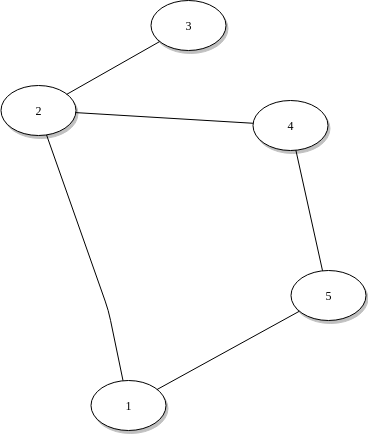
\includegraphics[width=\textwidth]{graf.png}
            \caption{Przykładowy graf}
            \label{example:graph}
        \end{figure}
    \end{minipage}
    \hspace{0.5cm}
    \begin{minipage}[b]{0.45\linewidth}
    \centering
    \begin{tabular}{|l|lllll}
        \hline
         & \multicolumn{1}{l|}{0} & \multicolumn{1}{l|}{1} & \multicolumn{1}{l|}{2} & \multicolumn{1}{l|}{3} & \multicolumn{1}{l|}{4} \\ \hline
        0 & 0 & 1 & 0 & 0 & 1 \\ \cline{1-1}
        1 & 1 & 0 & 1 & 1 & 0 \\ \cline{1-1}
        2 & 0 & 1 & 0 & 0 & 0 \\ \cline{1-1}
        3 & 0 & 1 & 0 & 0 & 1 \\ \cline{1-1}
        4 & 1 & 0 & 0 & 1 & 0 \\ \cline{1-1}
        \end{tabular}
        \caption{Przykładowa macierz sąsiedztwa}
        \label{example:table}
    \end{minipage}
    \end{table}

\paragraph{Macierz sąsiedztwa}
to sposób reprezentacji grafu w którym krawędzie reprezentowane są przez wartość 1 w komórce której pozycja odpowiada numerom wierzchołków.
Na rysunku \ref{example:graph} widzimy połączenie 1--2. Jest ono reprezentowane w tablicy \ref{example:table} poprzez 1 na pozycji 12 i 21.
Redundancja informacji spowodowana jest tym, że graf na rysunku \ref{example:graph} jest nieskierowany(nie można wyróżnić kierunku połączenia). 
Wady tej metody reprezentacji ujawniają się w przypadku grafów o małej liczbie połączeń. 
Ilość elementów w macierzy jest proporcjonalna do kwadratu ilości wierzchołków, gdy ilość połączeń jest znikoma duża część przechowywanych informacji to 0.


\begin{table}[H]
    \centering
    \begin{tabular}{|l|l|ll}
    \cline{1-3}
    \textbf{0} & 1 & \multicolumn{1}{l|}{4} &  \\ \hline
    \textbf{1} & 2 & \multicolumn{1}{l|}{0} & \multicolumn{1}{l|}{3} \\ \hline
    \textbf{2} & 1 &  &  \\ \cline{1-3}
    \textbf{3} & 1 & \multicolumn{1}{l|}{4} &  \\ \cline{1-3}
    \textbf{4} & 3 & \multicolumn{1}{l|}{0} &  \\ \cline{1-3}
    \end{tabular}
    \caption{Przykładowa lista sąsiedztwa}
    \label{example:list}
    \end{table}
\paragraph{Lista sąsiedztwa}
to sposób reprezentacji grafu przez wektor wektorów, gdzie indeksami pierwszej z nich(pogrubione cyfry w tablicy \ref{example:list}) oznaczany numer wierzchołka.
Pod każdym z indeksów znajduje się lista połączeń każdego wierzchołka. Zaletą tego rozwiązania jest stały czas dostępu do listy połączeń danego wierzchołka.

\subsubsection{Metody przeszukiwania}
\begin{description}
    \item [DFS] Depth first search -- przeszukiwanie w głąb\\ 
    Opiera się na przeszukiwaniu od korzenia wzdłuż każdej gałęzi tak głęboko, jak to możliwe zanim zacznie się cofać
    \item [BFS] Breath first search -- przeszukiwanie w szerz\\
    Opiera się na przeciwnej strategii do DFS i najpierw przeszukuje najpłycej położone węzły, zanim zejdzie głębiej.
    Z pośród rozważanych algorytmów jest to jedyny gwarantujący znalezienie najbliższego rozwiązania.
    \item [A*]  A star/gwiazdka -- heurystyczne przeszukiwanie\\
    Opiera się na zupełnie innym podejściu.
    W każdej iteracji wyznaczany jest koszt stanów, zgodnie z używaną metryką, i algorytm przeszukuje drzewo w pierwszej kolejności po węzłach o najniższym koszcie.
    \\
    Wykorzystane metryki to:
    \begin{description}
        \item [Manhattan] Dla każdego punktu liczona jest odległość od punktu docelowego
        \[d=\sum_{i=1}^{n} |x_i-x'_i|+|y_i-y'_i|\] 
        \item [Hamminga] Koszt zwiększa się wraz z każdym elementem będącym na złej pozycji
    \end{description}
\end{description}

\subsubsection{Pozostałe pojęcia}
\begin{description}
    \item [Cykliczność]
    Graf można zaklasyfikować jako cykliczny kiedy daje się w nim wytyczyć ścieżkę która zaczyna i kończy się w tym samym wierzchołku\cite{AlgDataStrucure}.
    Przykładowy graf z rysunku \ref{example:graph} ma cykl składający się z wierzchołków  1--0--4--3--1.
    \item [Droga]
    \item 
\end{description}

\subsection{Struktury danych}
\subsubsection{Kopiec}
\begin{table}[H]
    \begin{minipage}[b]{0.45\linewidth}\centering
        \begin{figure}[H]
            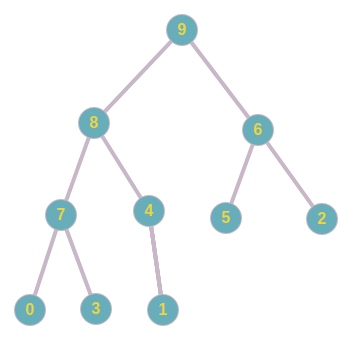
\includegraphics[width=\textwidth]{heap.png}
            \caption{Przykładowy graf drzewiasty}
            \label{heap:graph}
        \end{figure}
    \end{minipage}
    \hspace{0.5cm}
    \begin{minipage}[b]{0.45\linewidth}
    \centering
    \begin{tabular}{|l||l|l||l|l|l|l||l|l|l|}
        \hline
        9 & 8 & 6 & 7 & 4 & 5 & 2 & 0 & 3 & 1 \\ \hline
        \end{tabular}
        \caption{Kopiec powstały z drzewa rys.\ref{heap:graph}}
        \label{heap:table}
    \end{minipage}
    \end{table}

Kopiec jest strukturą danych reprezentującą drzewo binarne(spójny graf acykliczny) w postaci wektora\cite{STLAlgsVid}.
Kopce można podzielić na dwa typy\cite{IntroToAlgs}:
\begin{description}
    \item [Kopce max] gdzie wartość potomka jest zawsze mniejsza niż wartość rodzica.
    \item [Kopce min] gdzie wartość potomka jest zawsze większa niż wartość rodzica.
\end{description}

Rysunek \ref{heap:graph} przedstawia drzewo binarne które zostało przedstawione jako kopiec w tablicy \ref{heap:table}.
Kopiec można wyobrażać sobie jako kolejne poziomy drzewa binarnego dodawane na koniec tablicy.
Dla ułatwienia w tablicy \ref{heap:table} kolejne poziomy drzewa zostały oddzielone dodatkową linią.
Łatwo zauważyć, że pierwszy element nazywany też korzeniem(ang.root) jest w zależności od typu kopca jego największym(kopiec max) lub najniższym(kopiec min) elementem.
Struktura jest używana aby móc szybko otrzymać największy lub najmniejszy element kolekcji\cite{STLAlgsVid}.
\subsubsection{HashSet}
%To do
\section{Opis implementacji}
Implementację wykonano w języku Python3. 
Całość implementacji poza parserem parametrów i funkcją main() zamyka się w jednej klasie o długości ok. 200 linii, dlatego zrezygnowaliśmy z zamieszczania diagramu UML.

\section{Materiały i metody}

\begin{enumerate}
    \item  Przygotowanie danych
        \begin{itemize}
            \item Pobranie z platformy WIKAMP generatora układanek $4\times 4$
            \item Wygenerowanie przypadków testowych
        \end{itemize}
    \item Uruchomienie przygotowanego programu
        \begin{itemize}
            \item Pobranie z platformy WIKAMP skryptu uruchamiającego.
            \item Modyfikacja polecenia uruchamiającego w skrypcie.
            \item Uruchomienie skryptu
        \end{itemize}
    \item Analiza wyników i generowanie wykresów przy pomocy Jupyter Notobook'a
    \item Profit
\end{enumerate}

Celem zachowania wiarygodności pomiarów czasów program uruchomiono w środowisku tekstowym, jako process o największym priorytecie.
Podczas przetwarzania nie doszło do użycia pamięci swap ani throttlingu procesora.
\section{Wyniki}
\newgeometry{left=1cm,right=0.1cm,top=1cm, bottom=3cm}
\begin{figure}[H]
    \centering
    \begin{subfigure}[t]{0.45\textwidth}
        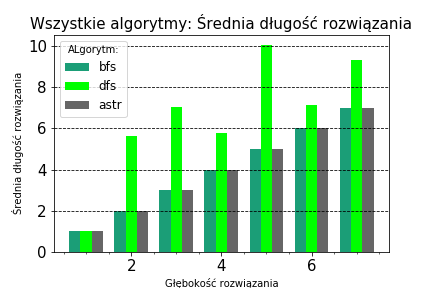
\includegraphics[width=\textwidth]{charts/ALL_path_length.png}
        \caption{Średnia długość rozwiązania}
        \label{ALL:path_length}
    \end{subfigure}
    ~ %add desired spacing between images, e. g. ~, \quad, \qquad, \hfill etc. 
      %(or a blank line to force the subfigure onto a new line)
    \begin{subfigure}[t]{0.45\textwidth}
        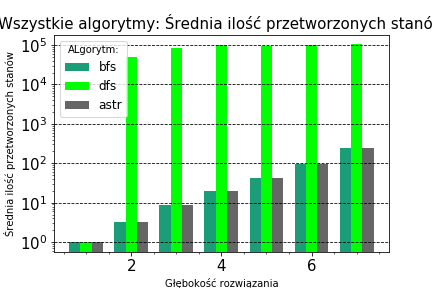
\includegraphics[width=\textwidth]{charts/ALL_processed.png}
        \caption{Średnia ilość przetworzonych stanów}
        \label{ALL:processed}
    \end{subfigure}
    \qquad
    ~ %add desired spacing between images, e. g. ~, \quad, \qquad, \hfill etc. 
    %(or a blank line to force the subfigure onto a new line)
    \begin{subfigure}[t]{0.45\textwidth}
        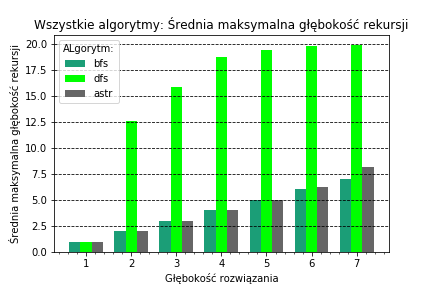
\includegraphics[width=\textwidth]{charts/ALL_recursed.png}
        \caption{Średnia maksymalna głębokość rekursji}
        \label{ALL:rescursed}
    \end{subfigure}
    \begin{subfigure}[t]{0.45\textwidth}
        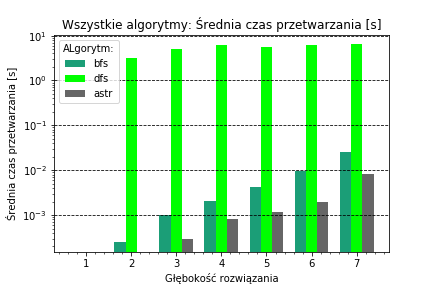
\includegraphics[width=\textwidth]{charts/ALL_time.png}
        \caption{Średni czas przetwarzania}
        \label{ALL:time}
    \end{subfigure}
    \begin{subfigure}[t]{0.45\textwidth}
        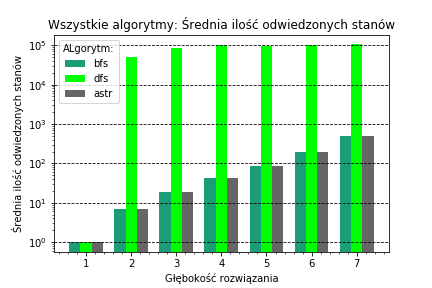
\includegraphics[width=\textwidth]{charts/ALL_visited.png}
        \caption{Średnia ilość odwiedzonych stanów}
        \label{ALL:visited}
    \end{subfigure}
    \caption{Porównanie wszystkich metod przeszukiwania}\label{col:all}
\end{figure}

\begin{figure}[H]
    \centering
    \begin{subfigure}[t]{0.45\textwidth}
        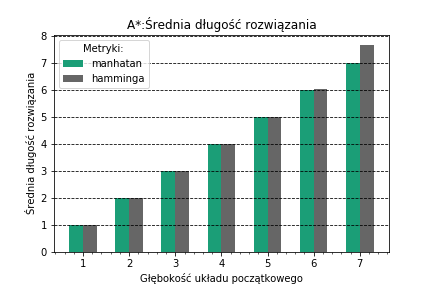
\includegraphics[width=\textwidth]{charts/ASTR_path_length.png}
        \caption{Średnia długość rozwiązania}
        \label{ASTR:path_length}
    \end{subfigure}
    ~ %add desired spacing between images, e. g. ~, \quad, \qquad, \hfill etc. 
      %(or a blank line to force the subfigure onto a new line)
    \begin{subfigure}[t]{0.45\textwidth}
        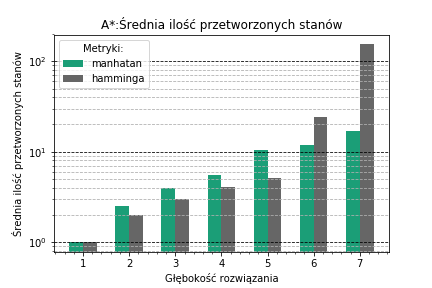
\includegraphics[width=\textwidth]{charts/ASTR_processed.png}
        \caption{Średnia ilość przetworzonych stanów}
        \label{ASTR:processed}
    \end{subfigure}
    \qquad
    ~ %add desired spacing between images, e. g. ~, \quad, \qquad, \hfill etc. 
    %(or a blank line to force the subfigure onto a new line)
    \begin{subfigure}[t]{0.45\textwidth}
        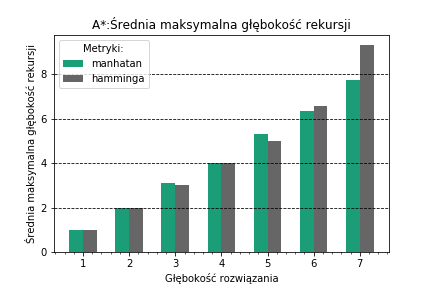
\includegraphics[width=\textwidth]{charts/ASTR_recursed.png}
        \caption{Średnia maksymalna głębokość rekursji}
        \label{ASTR:rescursed}
    \end{subfigure}
    \begin{subfigure}[t]{0.45\textwidth}
        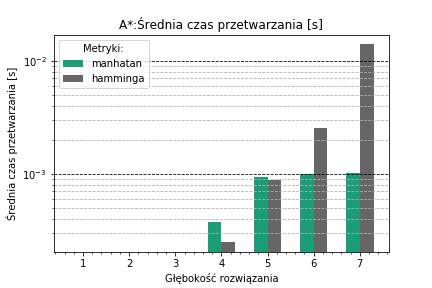
\includegraphics[width=\textwidth]{charts/ASTR_time.png}
        \caption{Średni czas przetwarzania}
        \label{ASTR:time}
    \end{subfigure}
    \begin{subfigure}[t]{0.45\textwidth}
        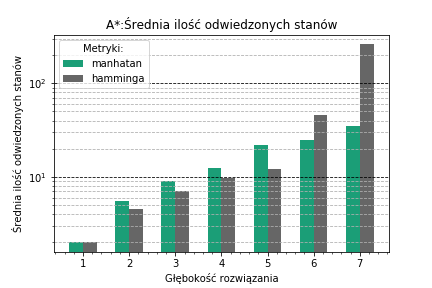
\includegraphics[width=\textwidth]{charts/ASTR_visited.png}
        \caption{Średnia ilość odwiedzonych stanów}
        \label{ASTR:visited}
    \end{subfigure}
    \caption{Porównanie wszystkich metod przeszukiwania}\label{coll:astr}
\end{figure}

\begin{figure}[H]
    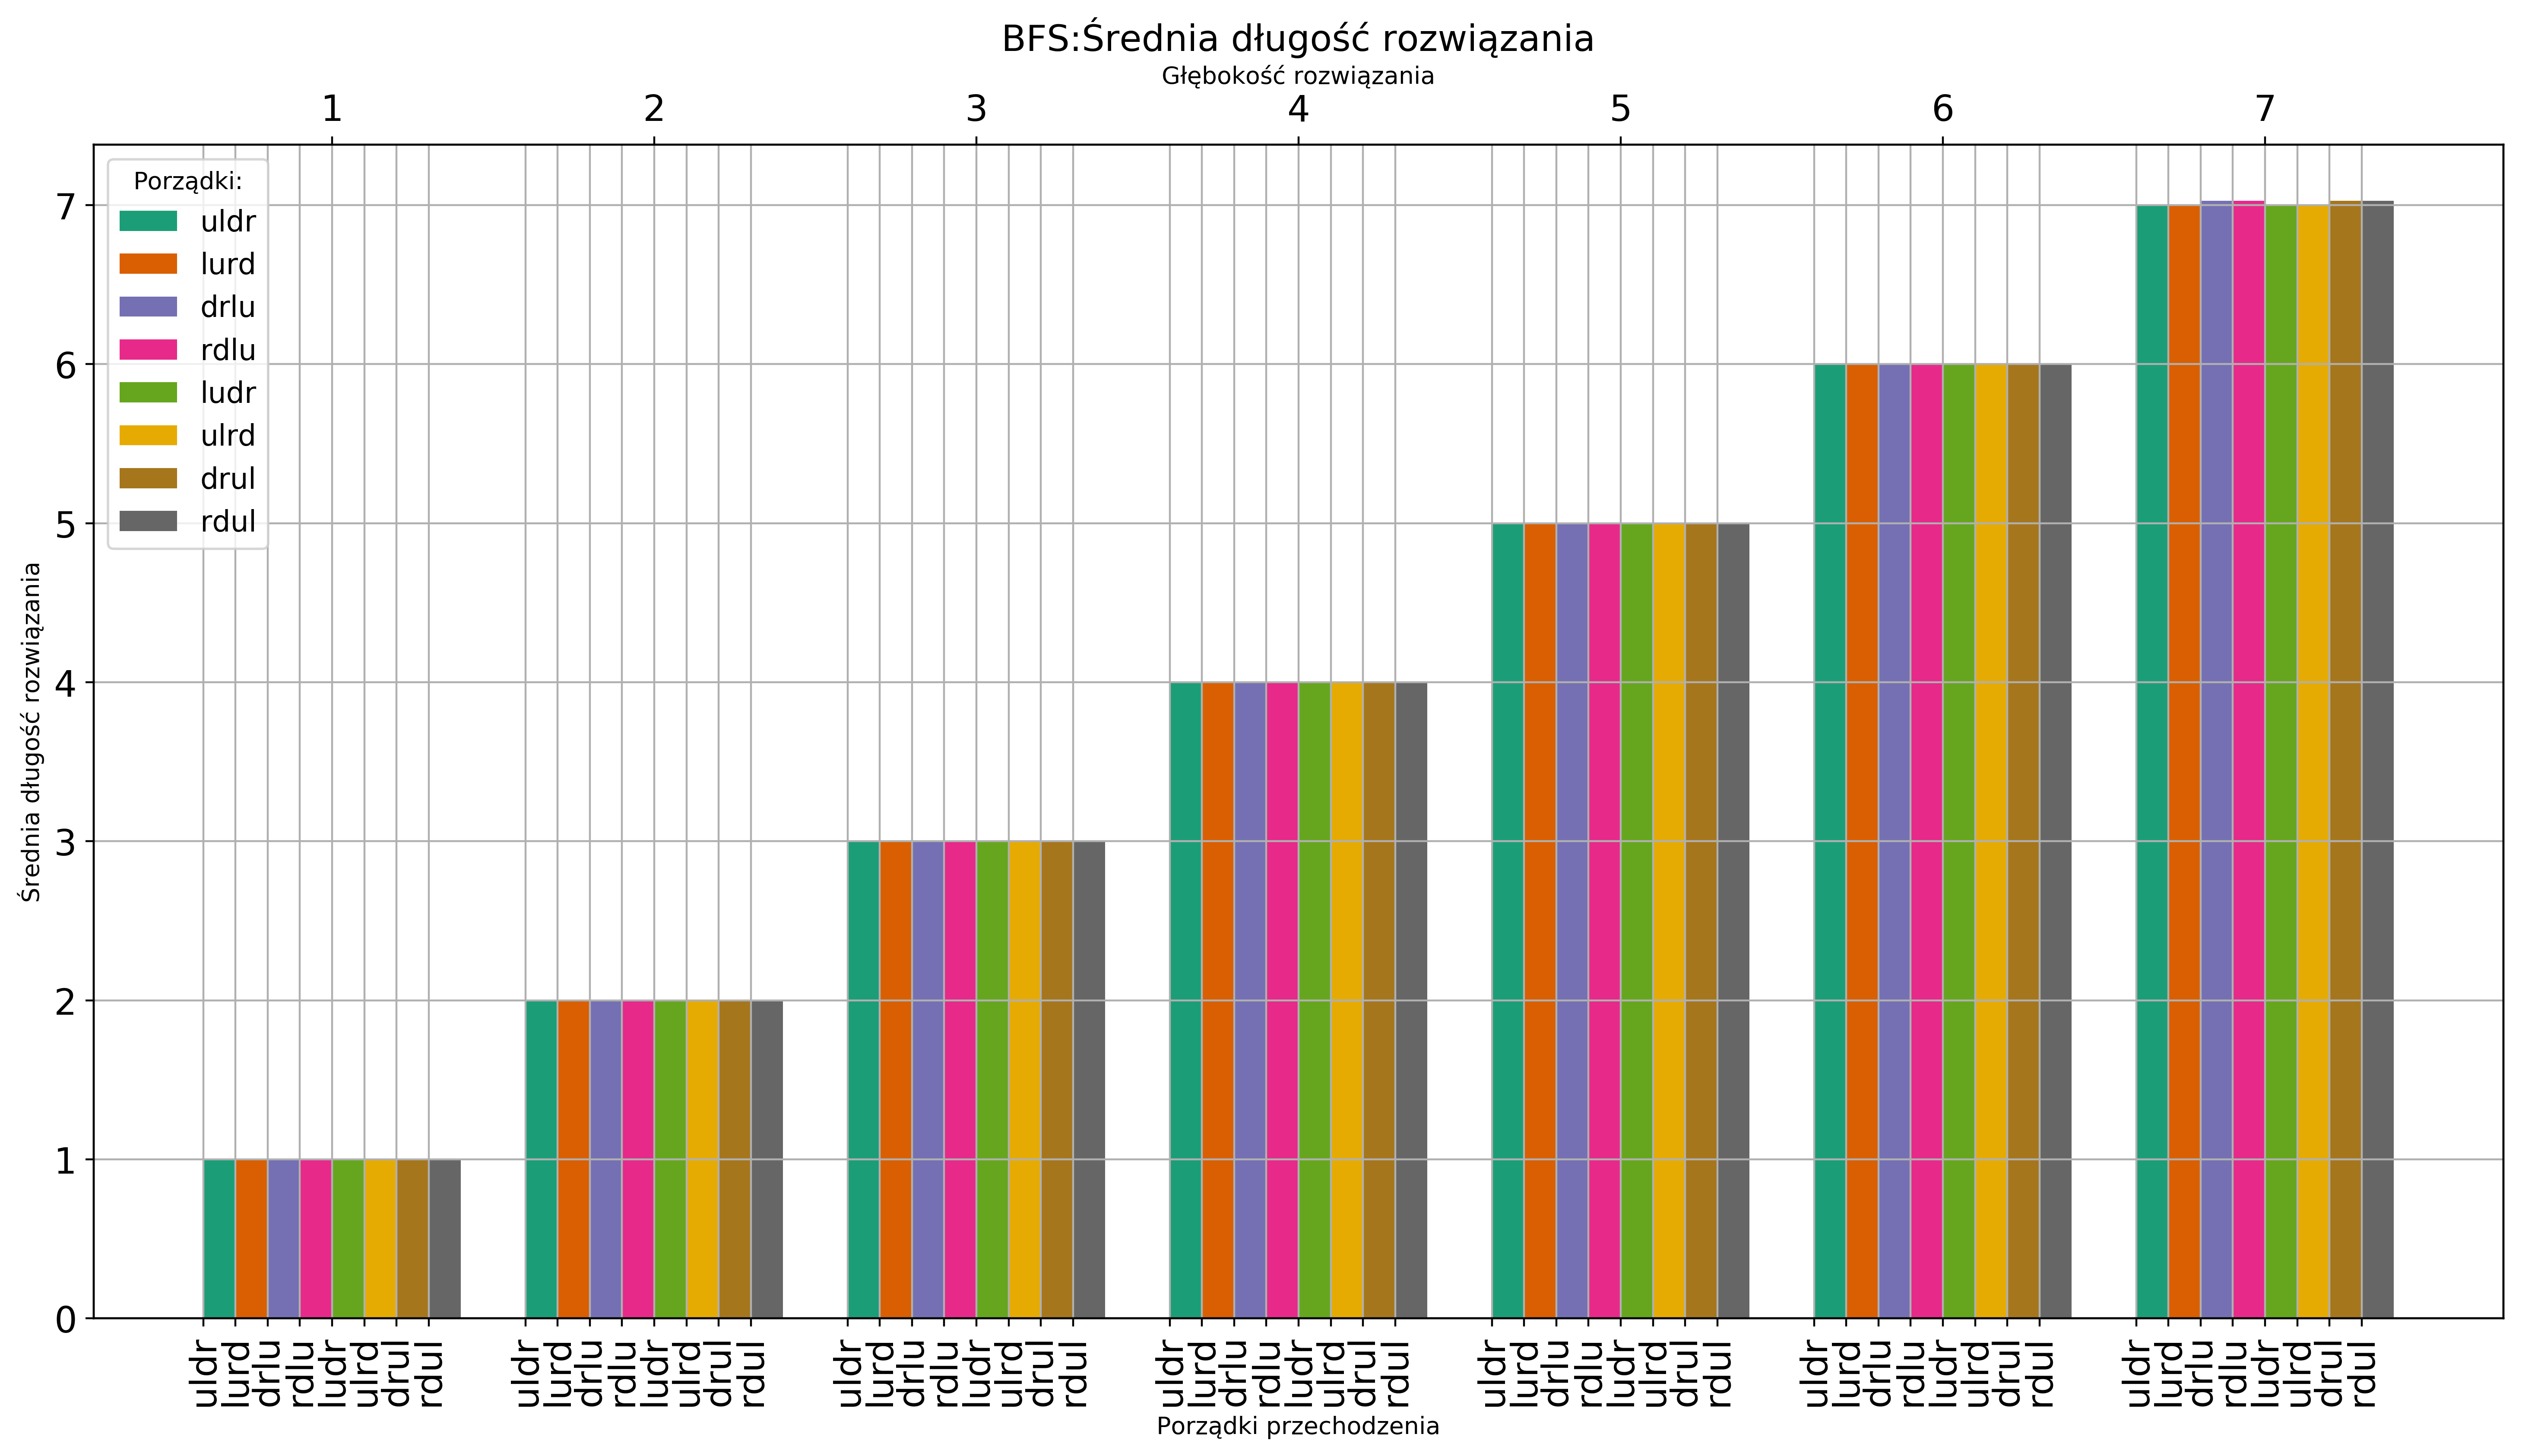
\includegraphics[width=\textwidth]{charts/BFS_path_length.png}
    \caption{BFS -- Średnia długość rozwiązania}
    \label{BFS:path_length}
    \vspace{0.2cm}
    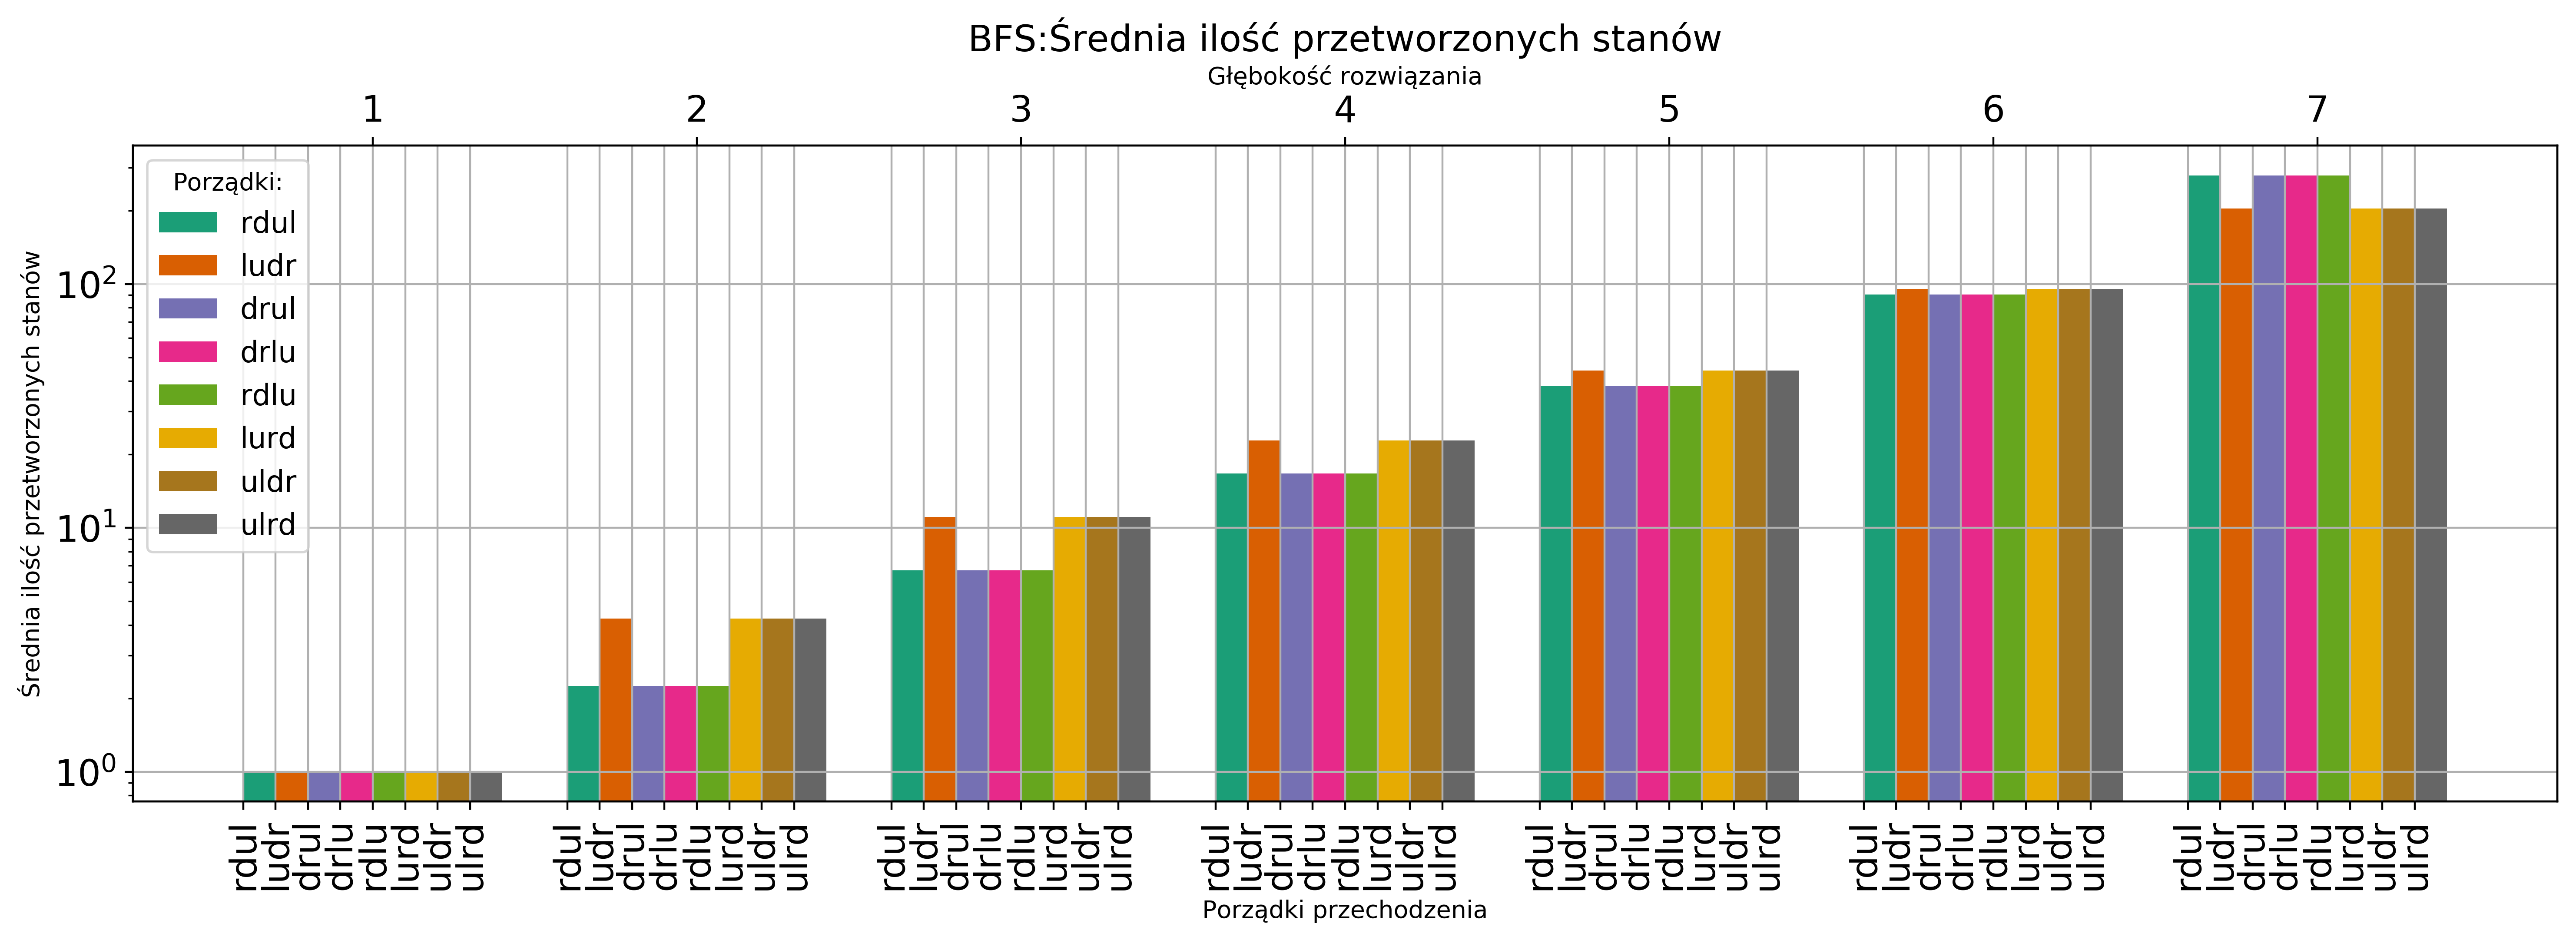
\includegraphics[width=\textwidth]{charts/BFS_processed.png}
    \caption{BFS -- Średnia ilość przetworzonych stanów}
    \label{BFS:processed}
    \vspace{0.2cm}
    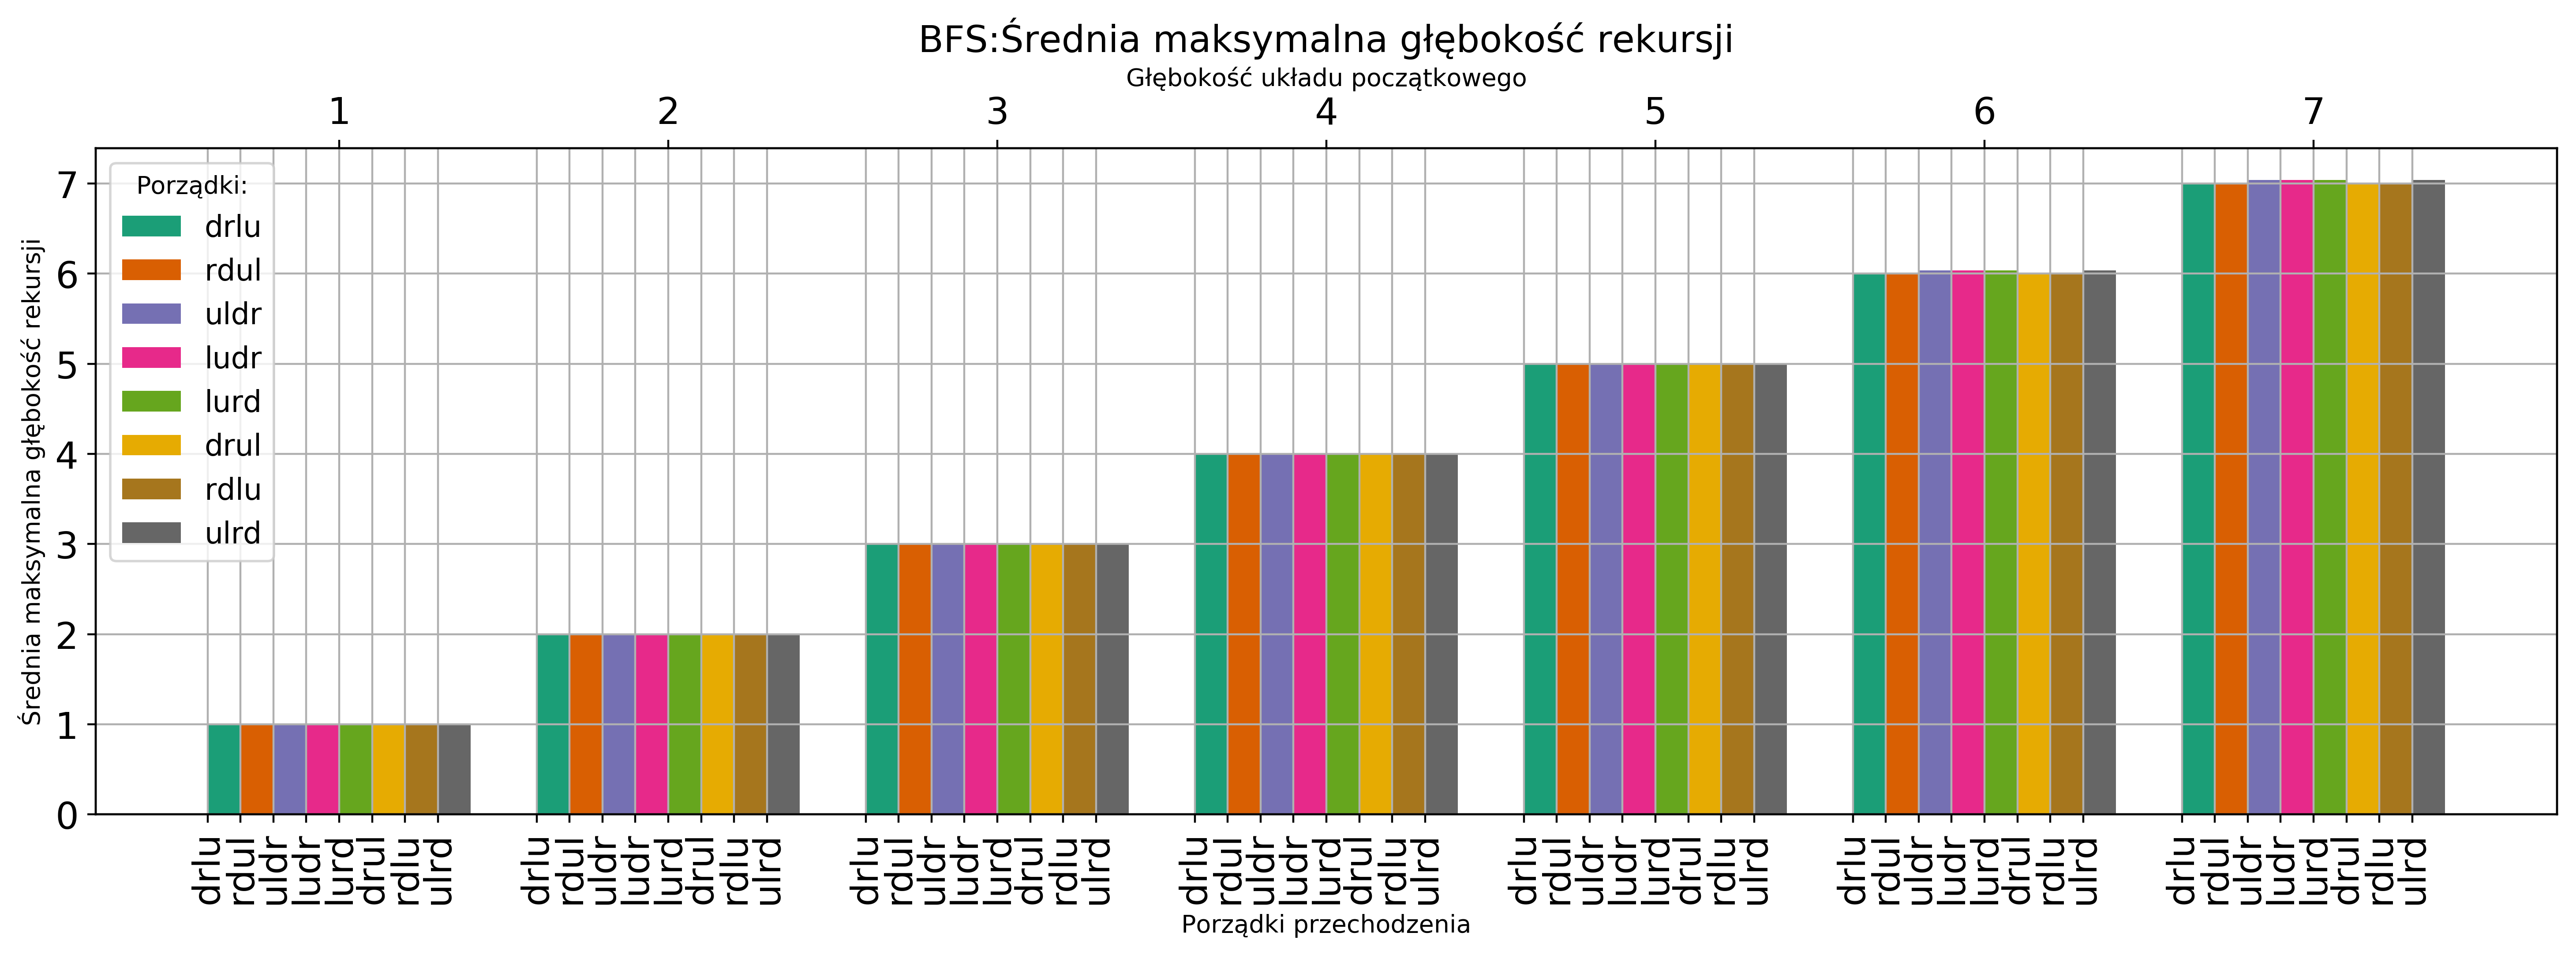
\includegraphics[width=\textwidth]{charts/BFS_recursed.png}
    \caption{BFS --  Średnia maksymalna głębokość rekursji}
    \label{BFS:recursed}

\end{figure}

\begin{figure}[H]
    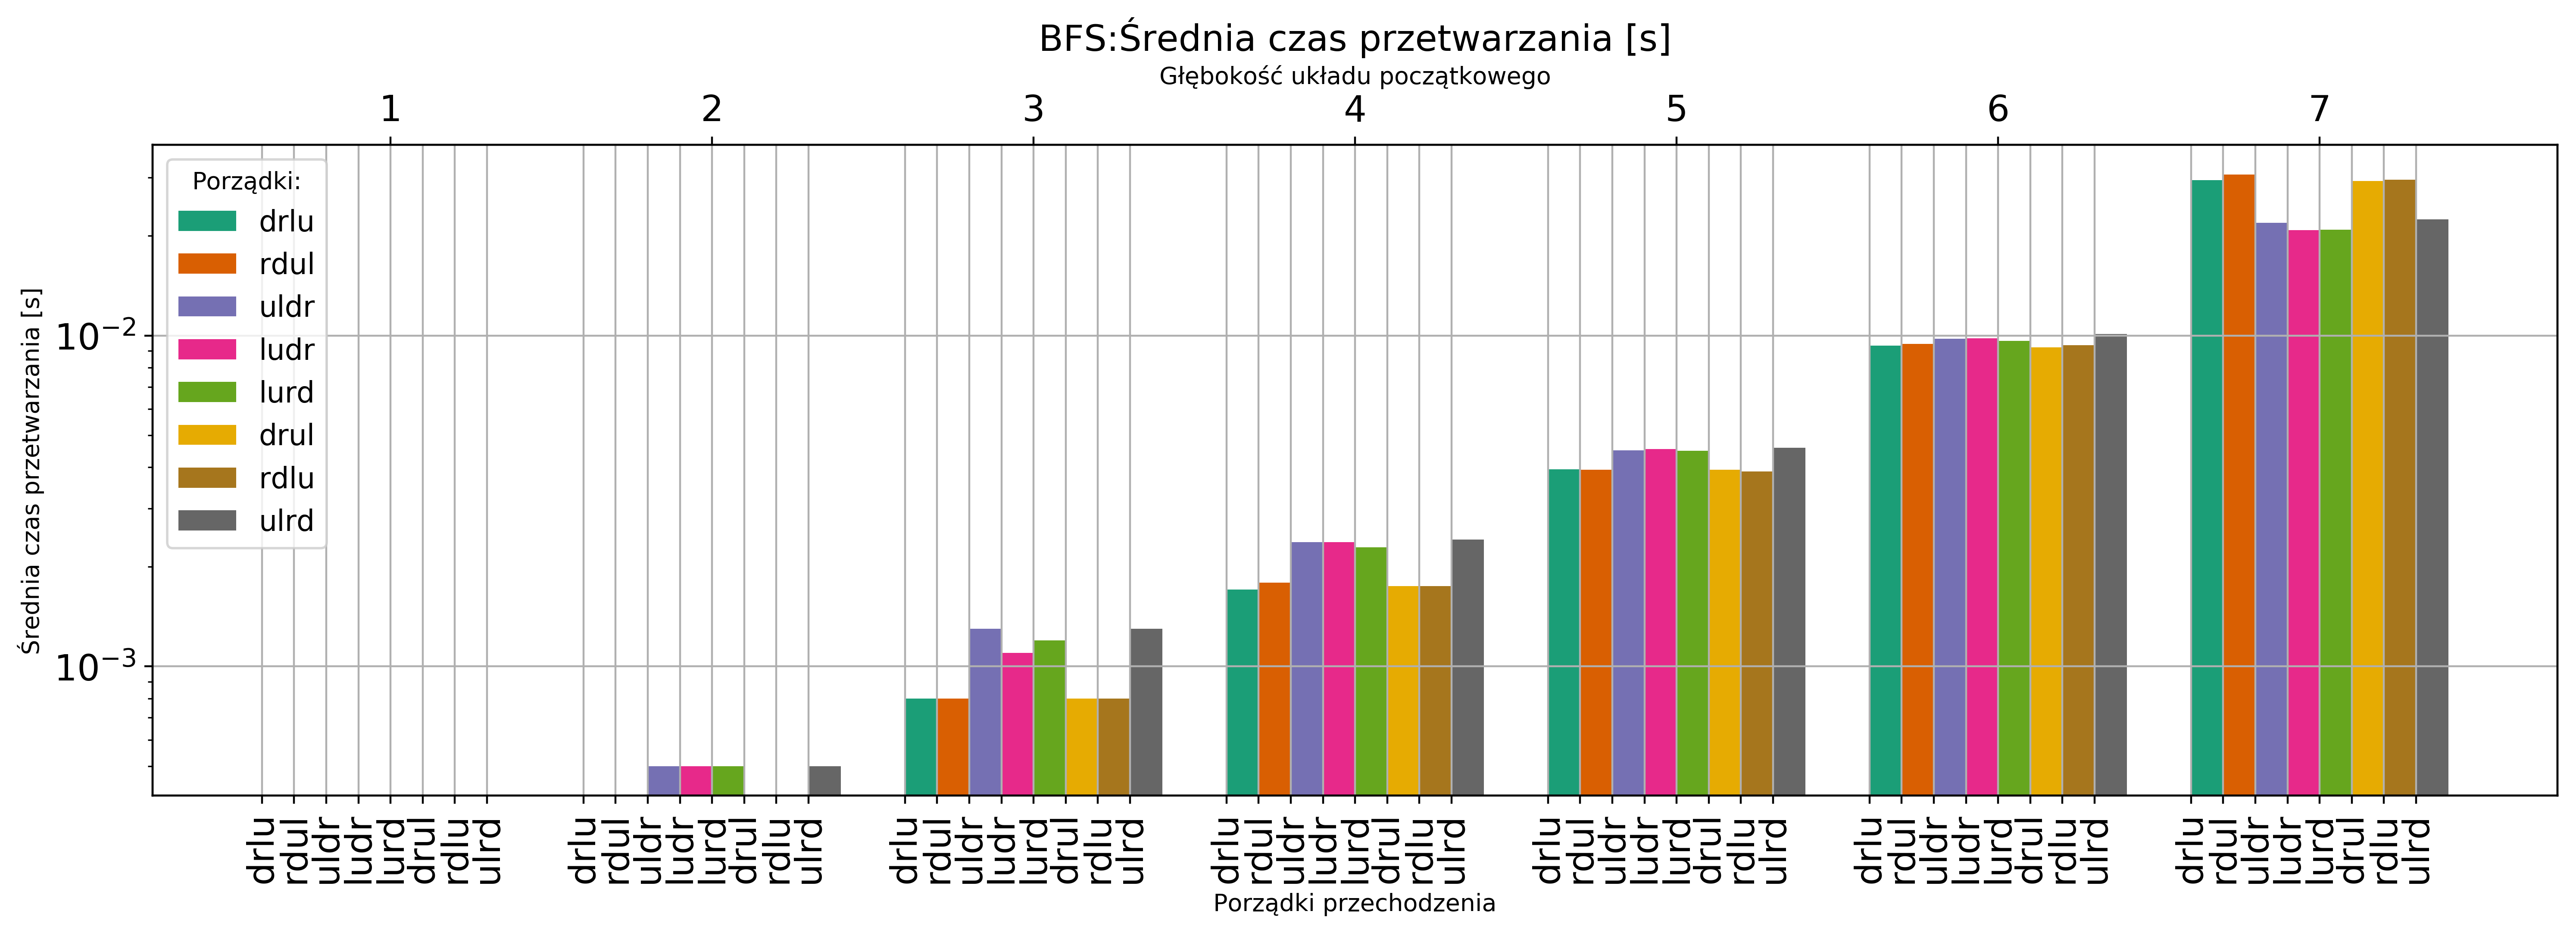
\includegraphics[width=\textwidth]{charts/BFS_time.png}
    \caption{BFS -- Średni czas przetwarzania}
    \label{BFS:time}
    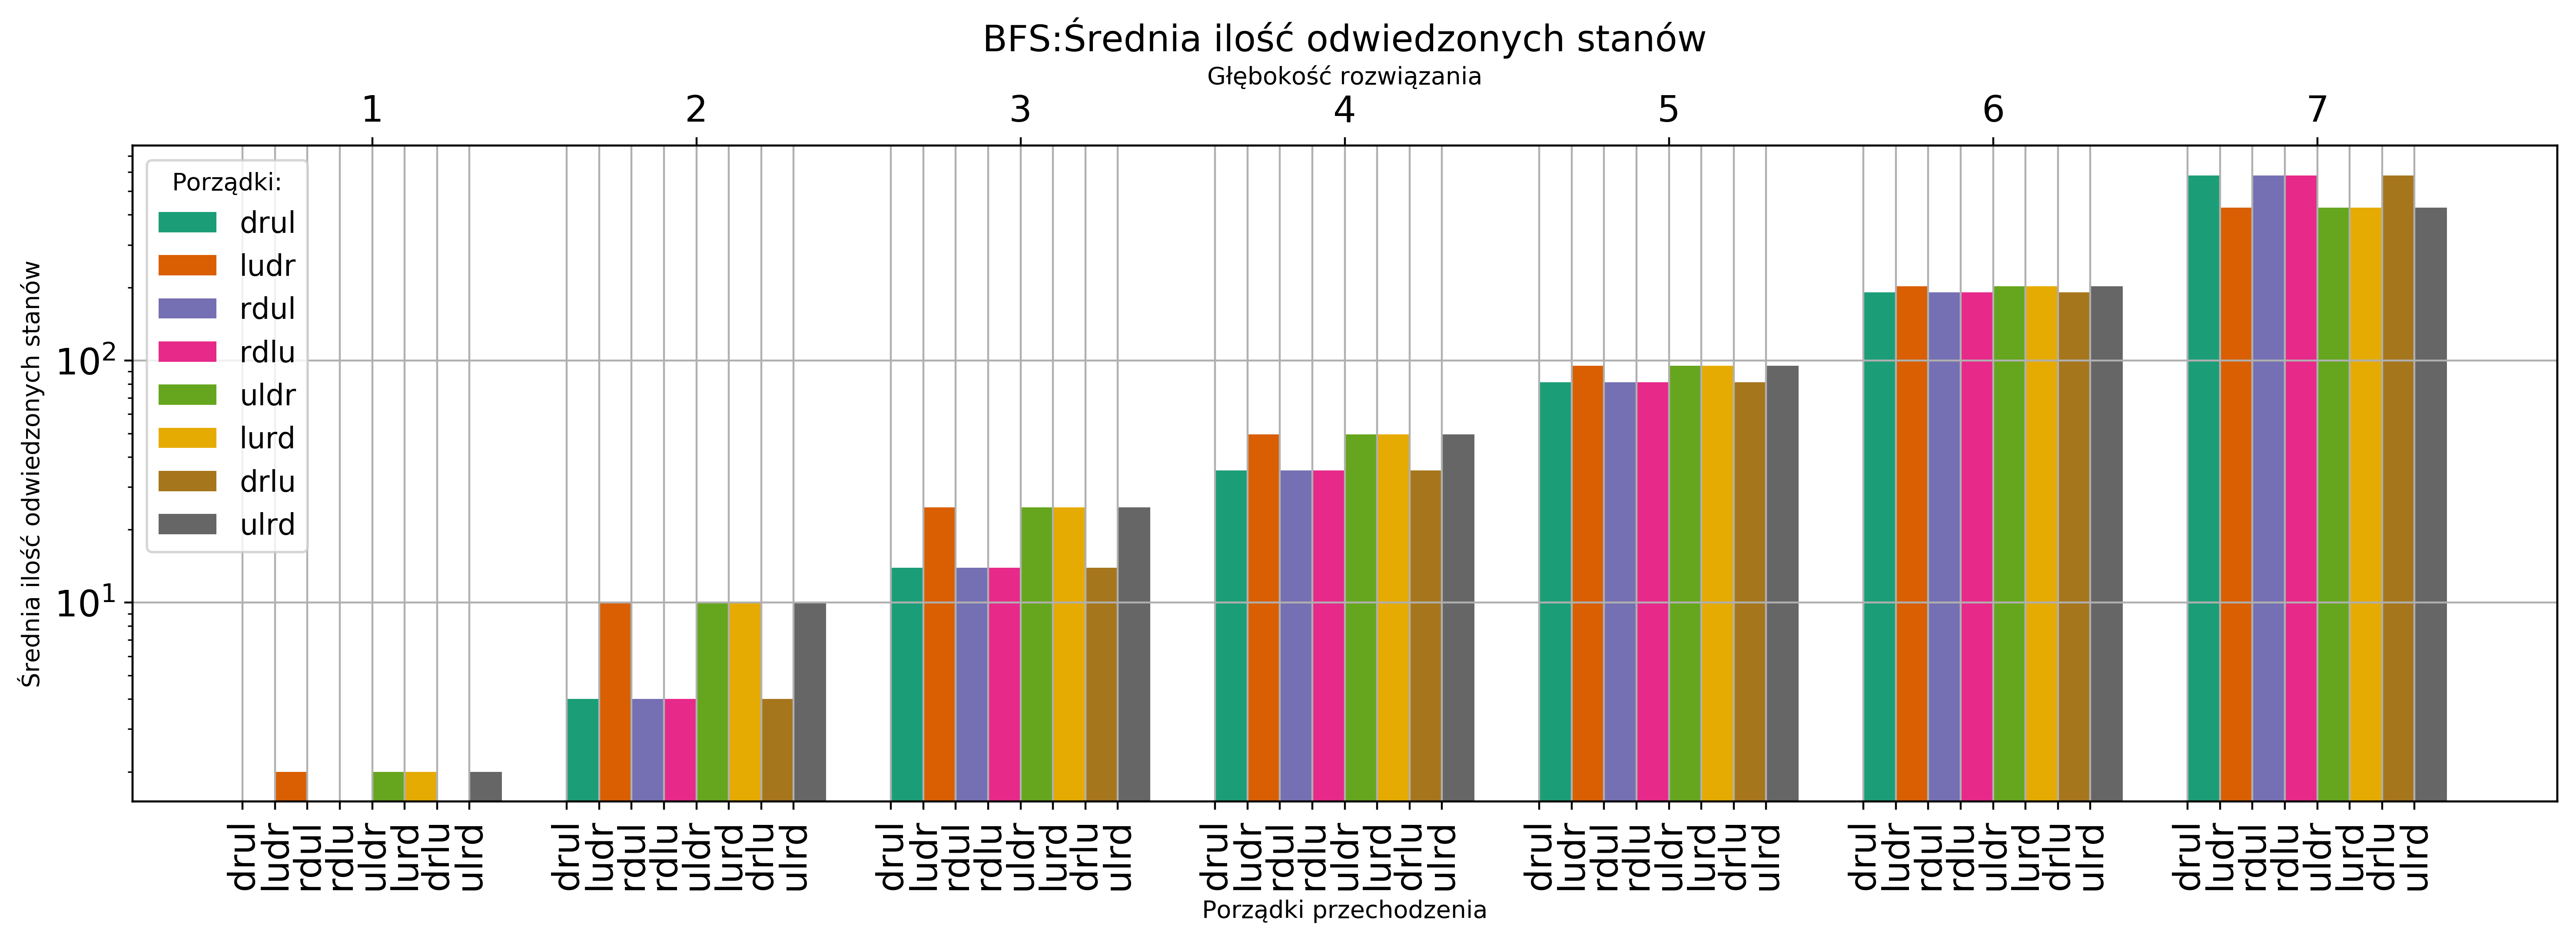
\includegraphics[width=\textwidth]{charts/BFS_visited.png}
    \caption{BFS -- Średnia ilość odwiedzonych stanów}
    \label{BFS:visited}
\end{figure}

\begin{figure}[H]
    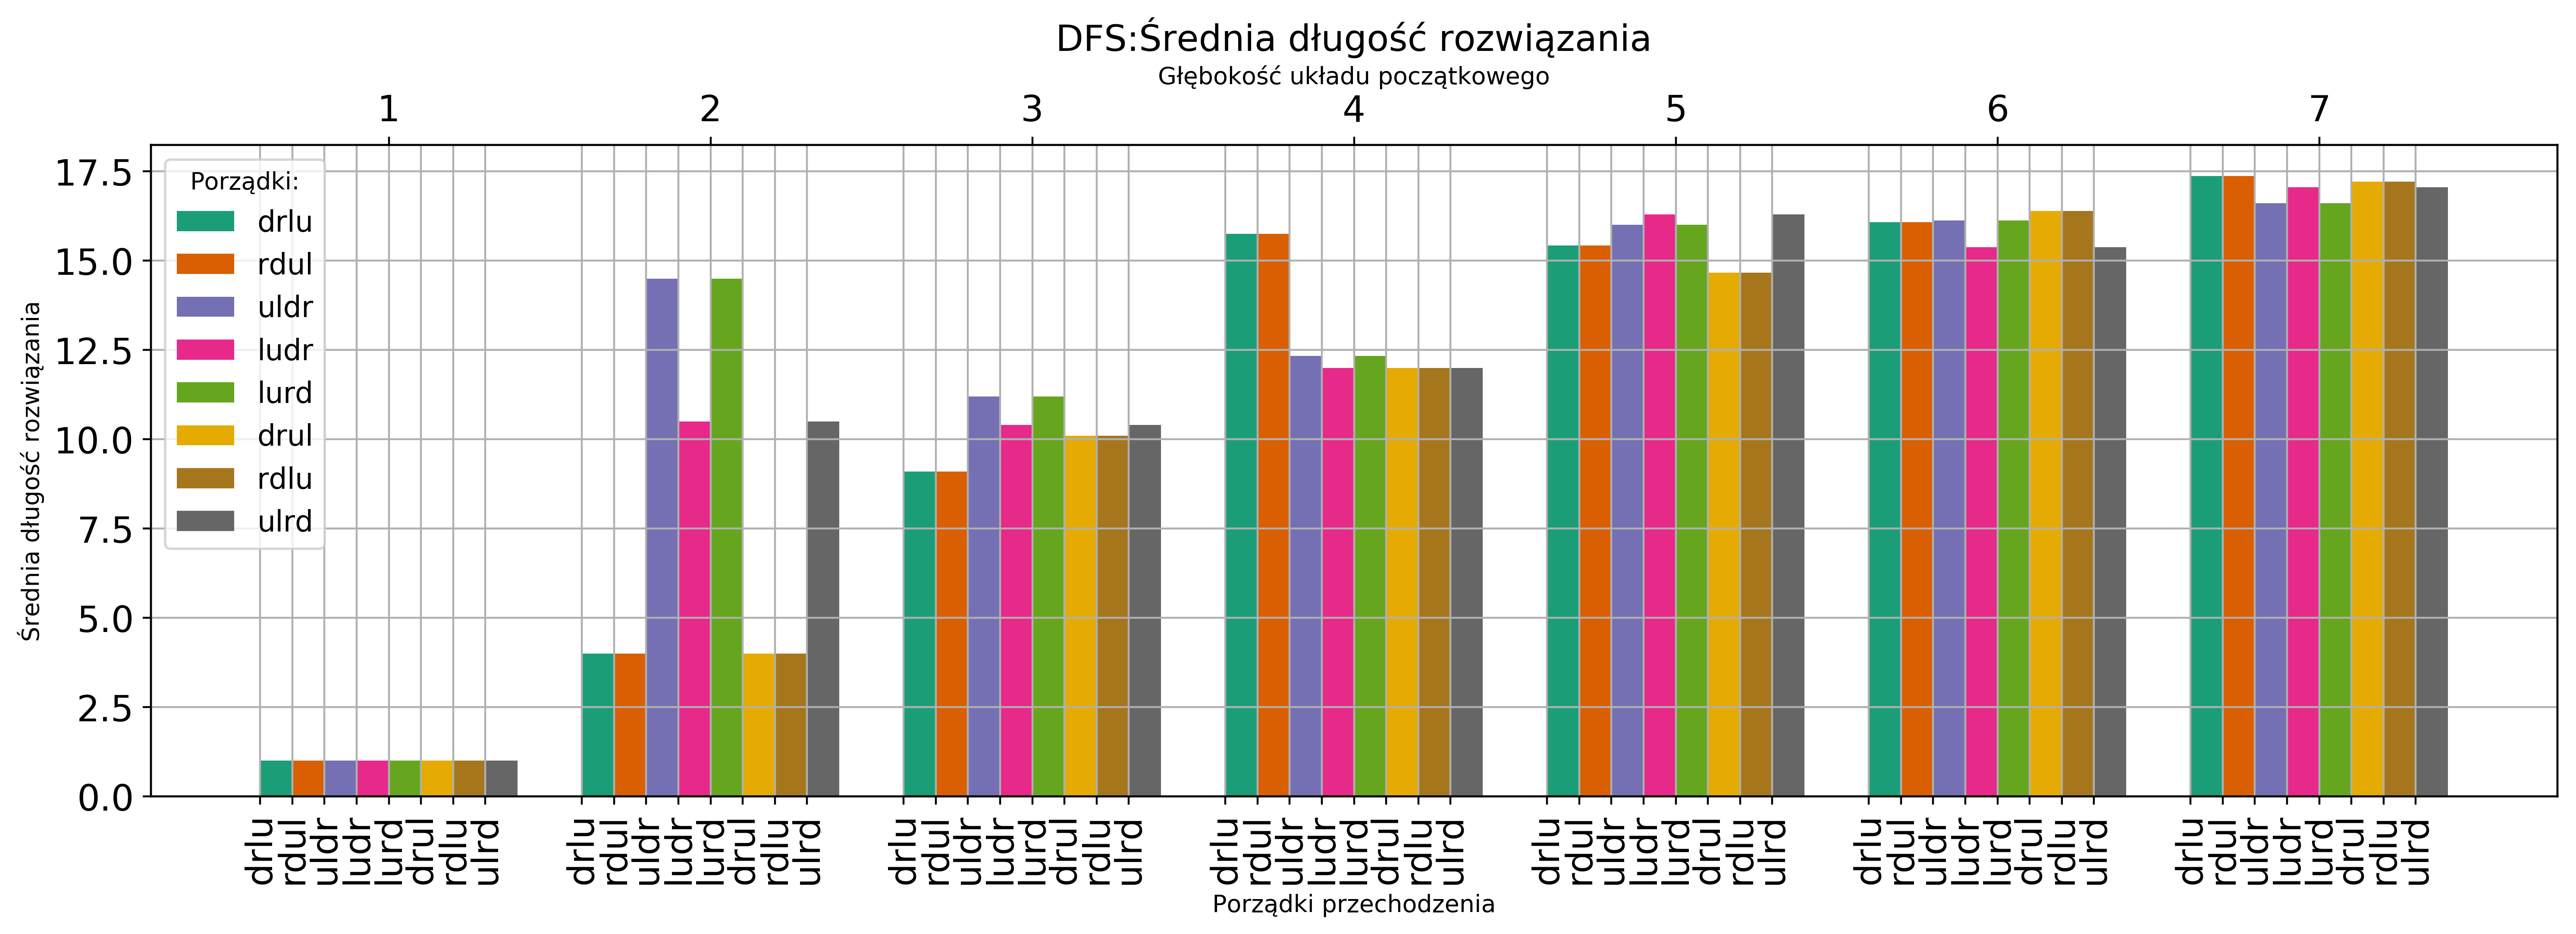
\includegraphics[width=\textwidth]{charts/DFS_path_length.png}
    \caption{DFS -- Średnia długość rozwiązania}
    \label{DFS:path_length}
    \vspace{0.2cm}
    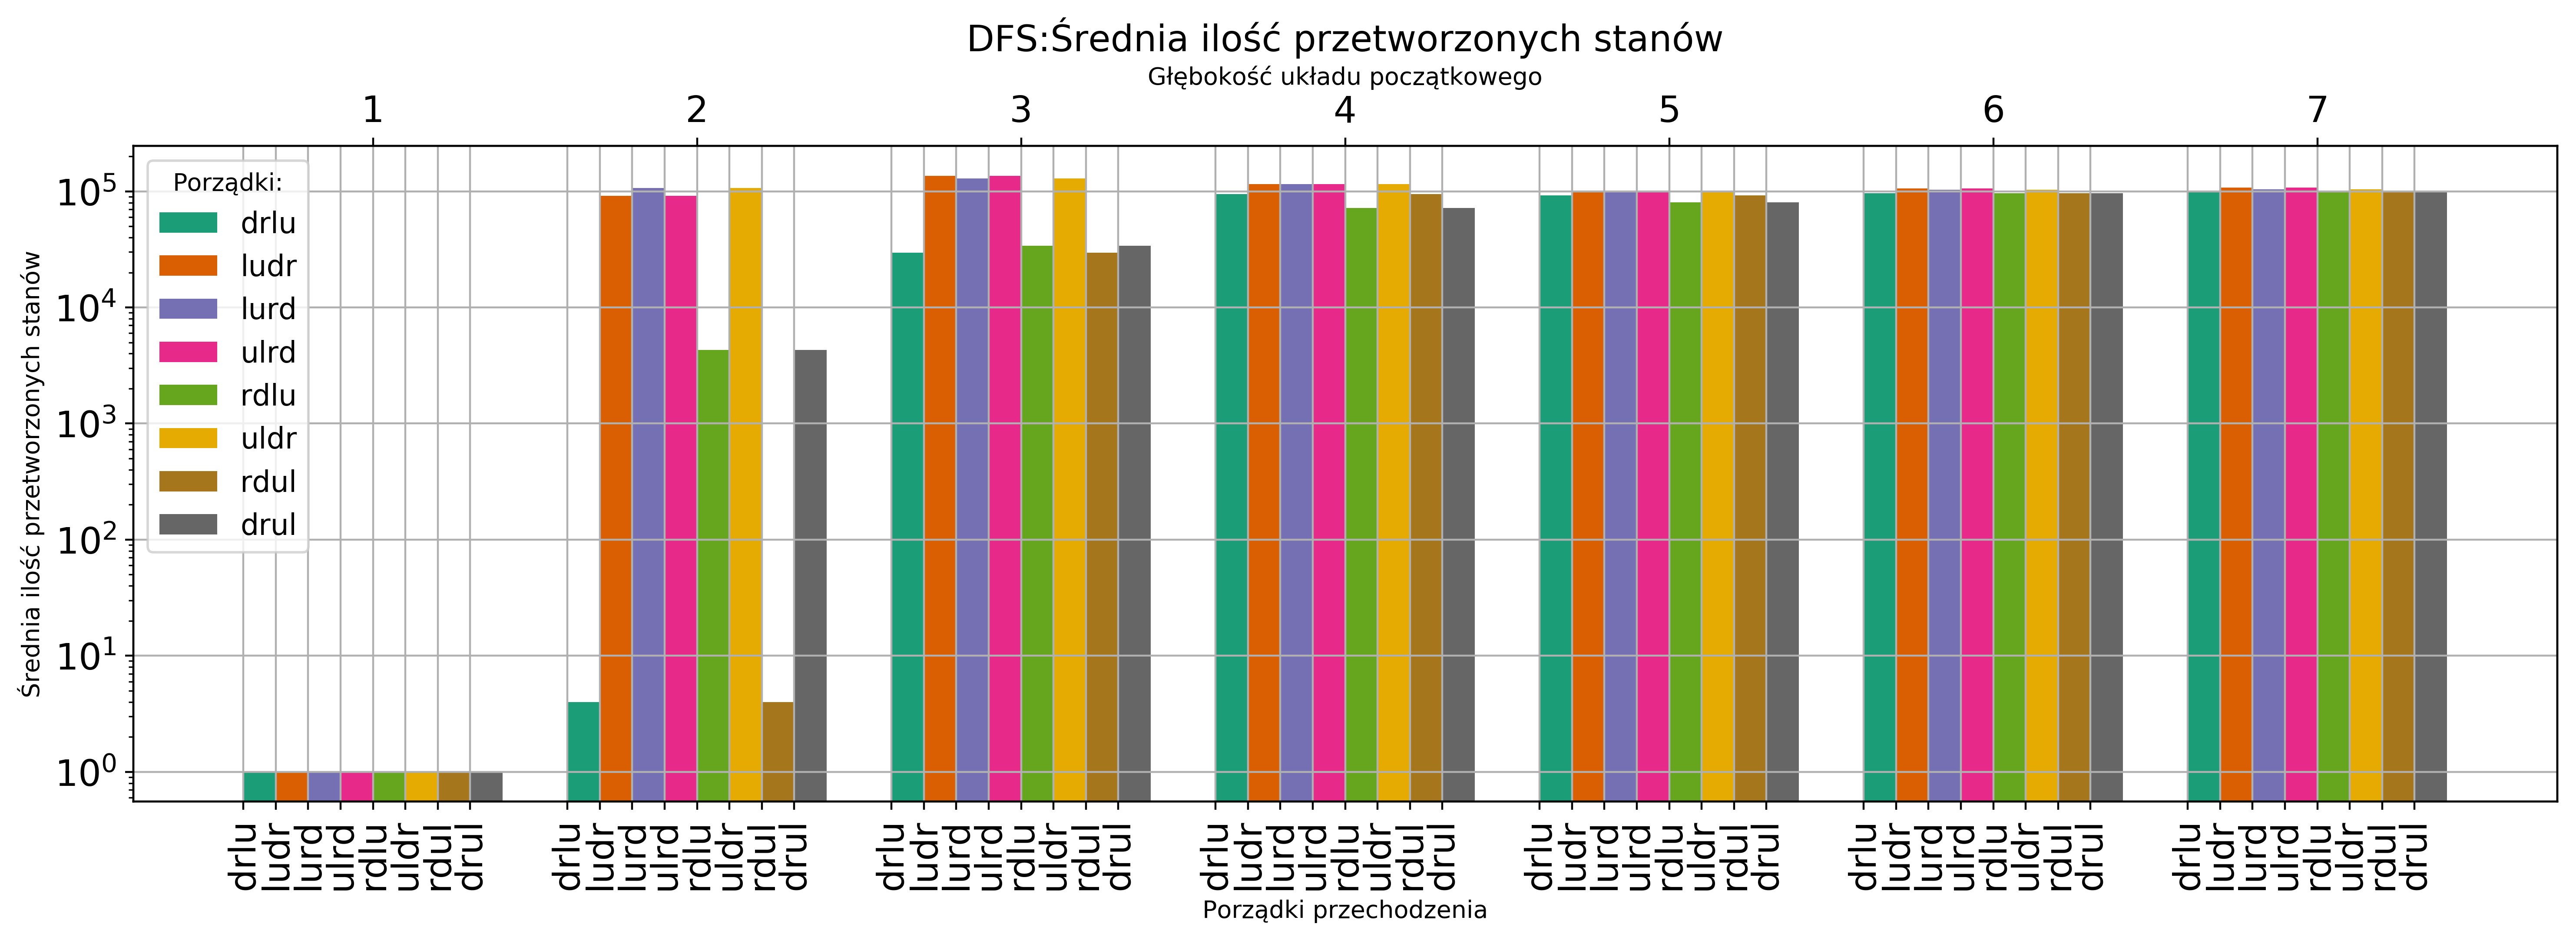
\includegraphics[width=\textwidth]{charts/DFS_processed.png}
    \caption{DFS -- Średnia ilość przetworzonych stanów}
    \label{DFS:processed}
    \vspace{0.2cm}
    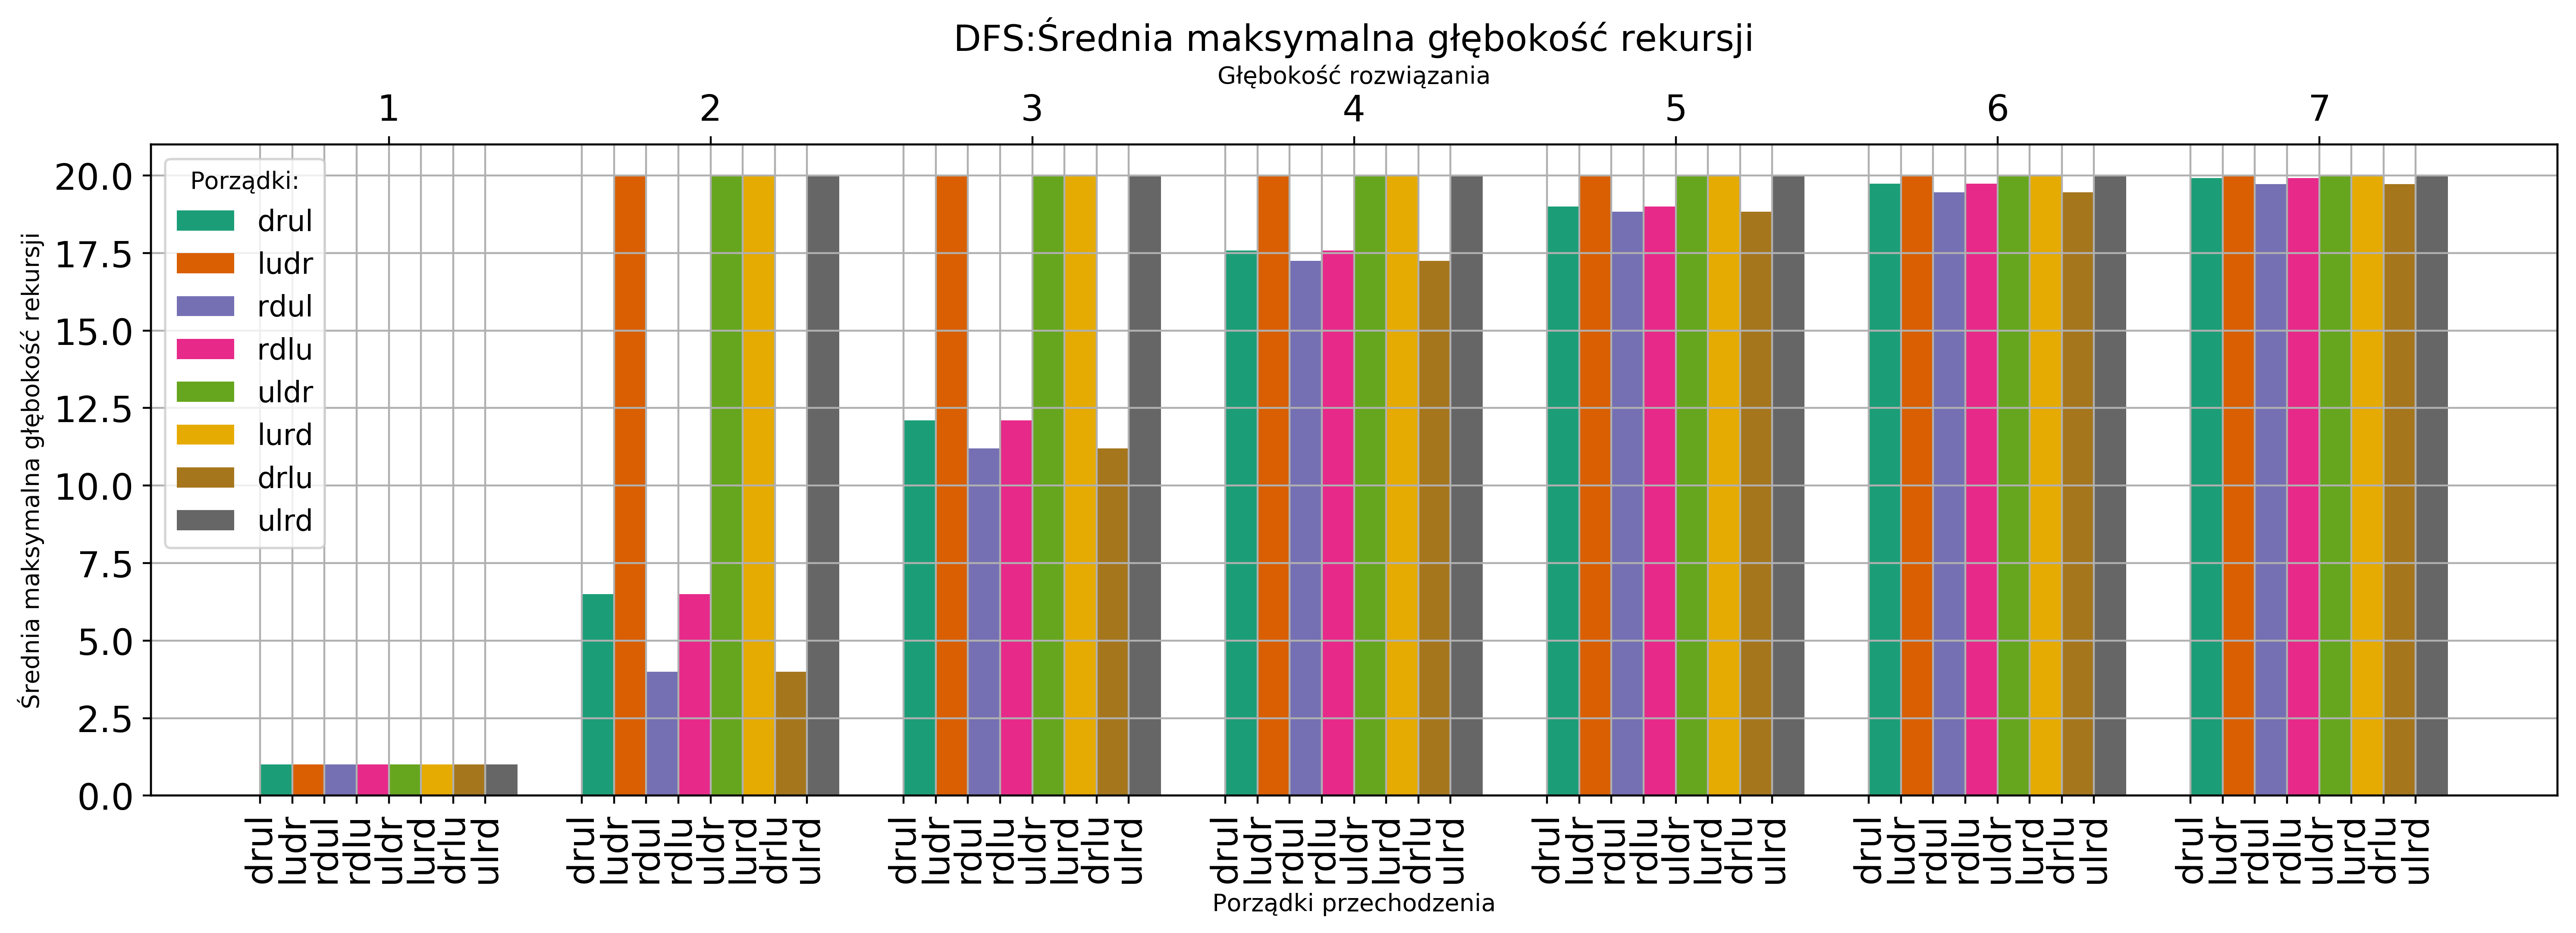
\includegraphics[width=\textwidth]{charts/DFS_recursed.png}
    \caption{DFS --  Średnia maksymalna głębokość rekursji}
    \label{DFS:recursed}

\end{figure}

\begin{figure}[H]
    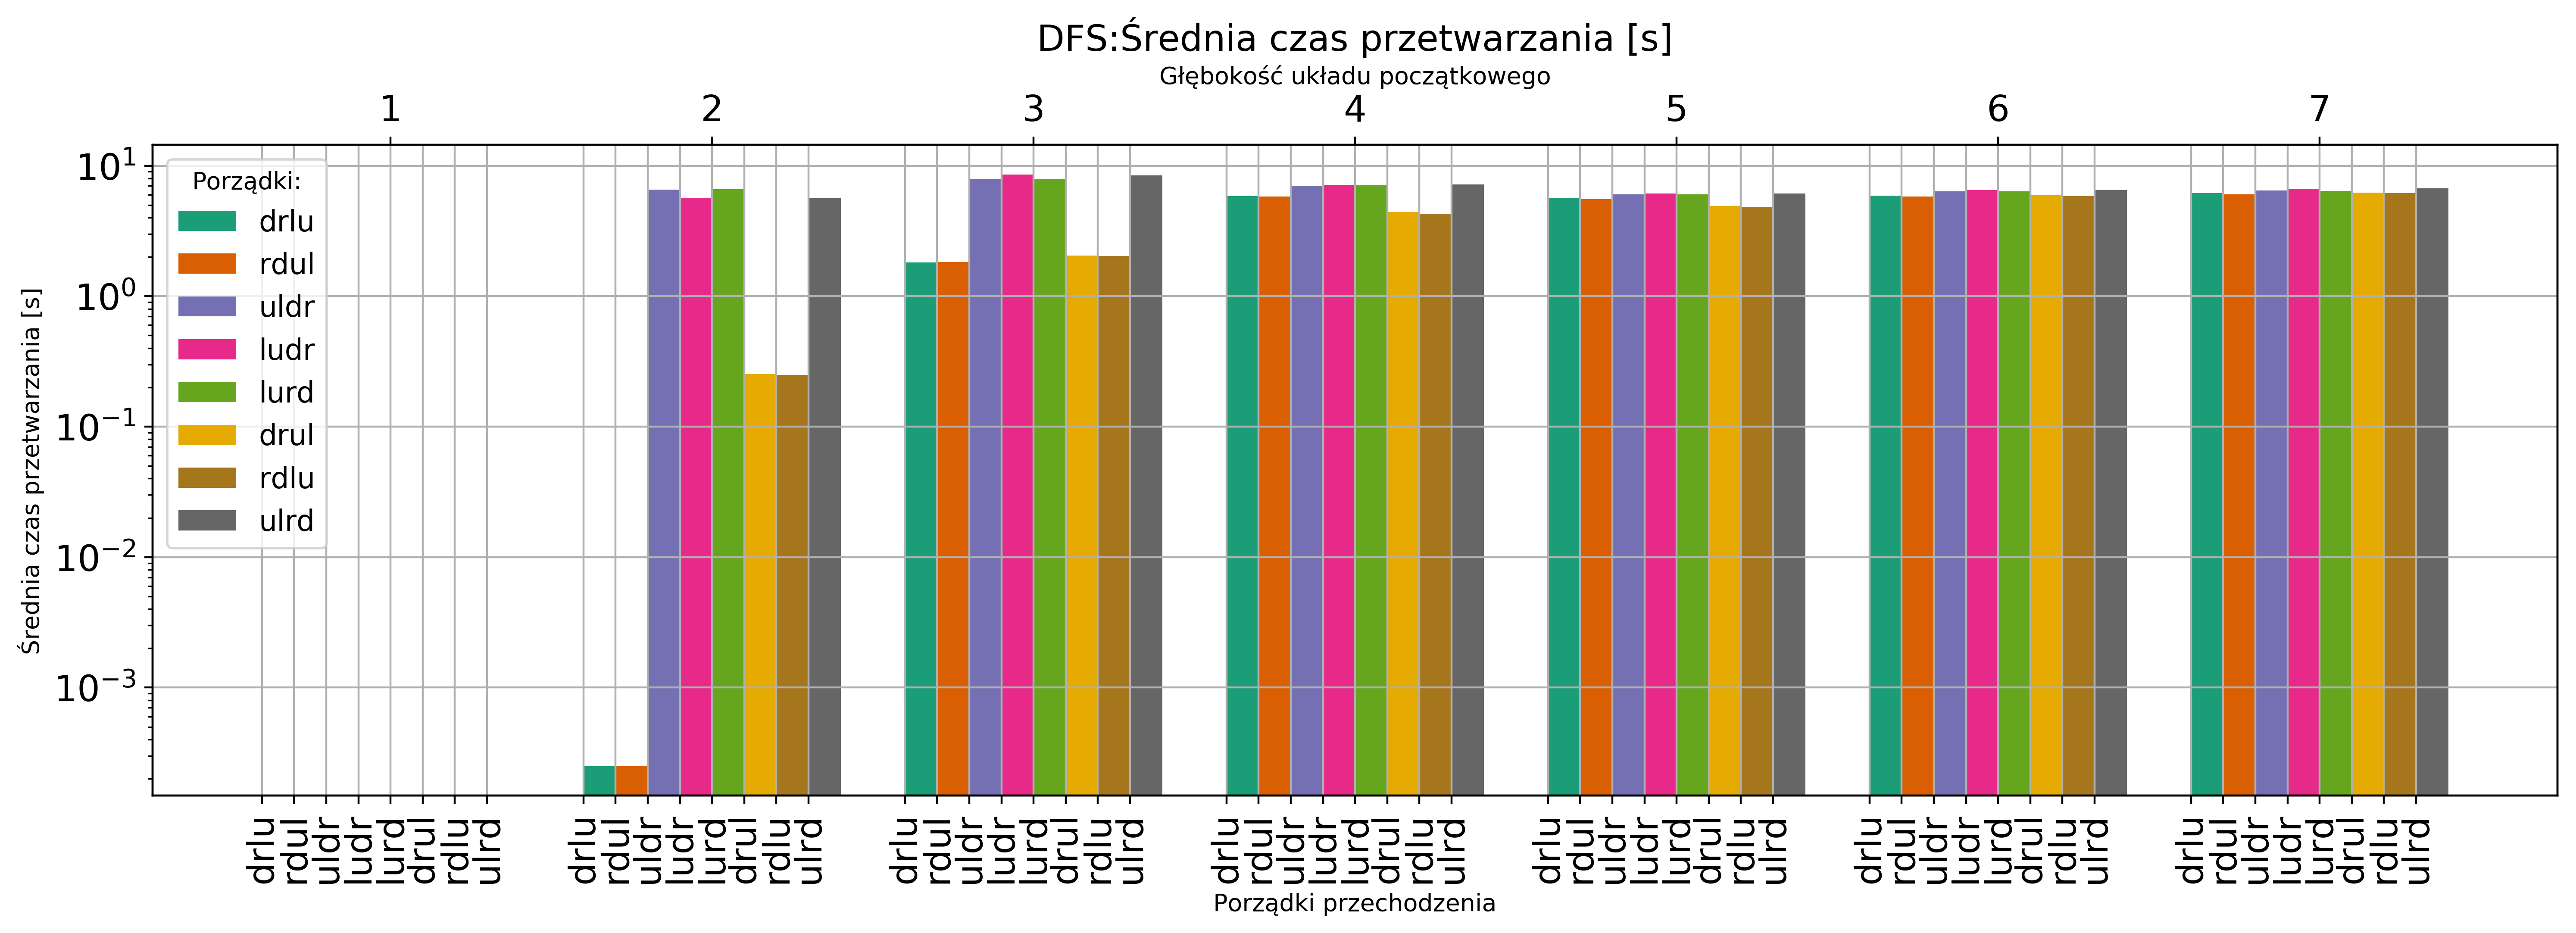
\includegraphics[width=\textwidth]{charts/DFS_time.png}
    \caption{DFS -- Średni czas przetwarzania}
    \label{DFS:time}
    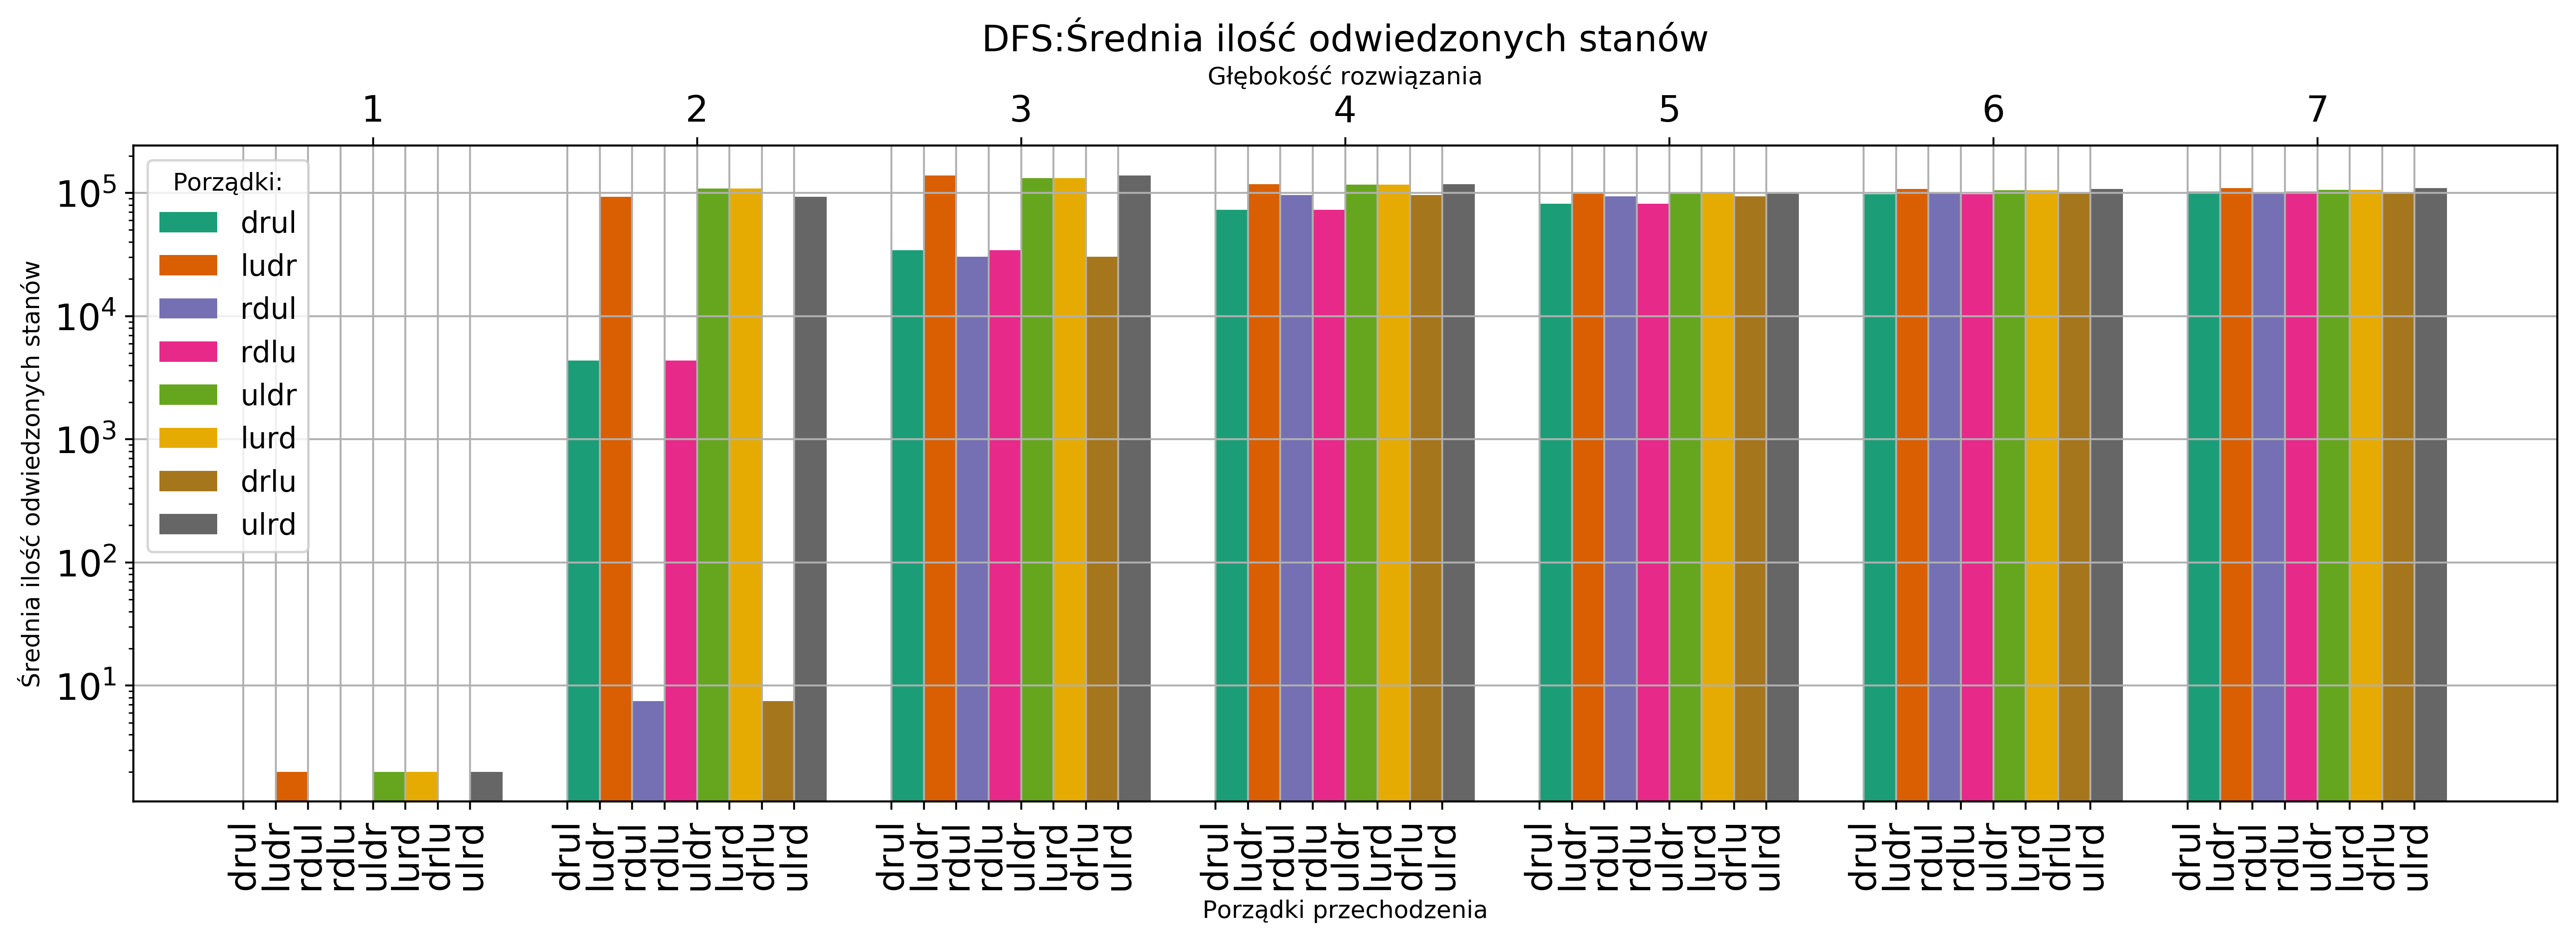
\includegraphics[width=\textwidth]{charts/DFS_visited.png}
    \caption{DFS -- Średnia ilość odwiedzonych stanów}
    \label{DFS:visited}
\end{figure}
\restoregeometry
Rysunek \ref{col:all} pokazuje, że A* jest najlepszy jeśli chodzi o ilość przetworzonych stanów i czas rozwiązania. DFS jest zawsze najmniej optymalny.
Przedstawione na rysunku \ref{coll:astr} wyniki metryk algorytmu A* wskazują iż metryka Hamminga działa lepiej dla rozwiązań położonych płycej niż 6.
Wyniki zaprezentowane na rysunkach \ref{BFS:path_length}, \ref{BFS:processed}, \ref{BFS:recursed}, \ref{BFS:visited} i \ref{BFS:time} wskazują na brak korelacji między wynikami a użytym porządkiem sąsiedztwa.
W przypadku algorytmu DFS w 1184 przypadkach rozwiązanie nie zostało odnalezione przyjęto wtedy, że długość ścieżki jest równa głębokości rekurencji, czyli 20.

\section{Dyskusja}
\subsection{Porównanie wszystkich algorytmów}
Najbardziej oczywistym wnioskiem płynącym z rysunku \ref{col:all} jest to iż, z pośród rozważanych algorytmów DFS jest średnio najmniej optymalny.
Otrzymane rezultaty tego sposobu rozwiązania, wymusiły użycie skali połlogarytmicznej, aby utrzymać czytelność wykresów.
Ilustracja \ref{ALL:path_length} pokazuje, że DFS średnio odnajduje rozwiązanie dalekie od optymalnego.
Na diagramie \ref{ALL:rescursed} widać, że osiągana głębokość przeszukiwania nie zwiększa się znacząco, jeśli rozwiązanie położone jest w odległości 4 lub większej.
Powodem tego jest odgórnie nałożony limit maksymalnej głębokości rekursji wynoszący w naszym przypadku 20.
Na rysunkach \ref{ALL:processed} i \ref{ALL:visited} widać, że znacznie większa głębokość rekursji koreluje z wielokrotnie wyższymi statystykami wierzchołków odwiedzonych i przetworzonych.
Potrzeba przetworzenia znacznie większej części przestrzeni stanów objawi się też znacznie dłuższym czasem wykonania widocznymi na \ref{ALL:time}.
Nieoptymalność przeszukiwania w głąb jest zgodna z intuicją autorów.
Szanse na to, że rozwiązanie położone jest głębiej, niż szerzej wydają się być małe, biorąc pod uwagę jak szybko rozszerza graf przestrzeni stanów.


Przeszukiwanie w szerz będące metodą brute-force szukającą najpłytszego rozwiązania przeszukując graf stanów poziom po poziomie, zawsze osiąga lepsze wyniki niż DFS.
Na rysunku \ref{ALL:path_length} i \ref{ALL:rescursed} widać, że BFS zawsze odnajduje najpłytsze rozwiązanie. Na wykresach \ref{ALL:processed} i \ref{ALL:visited} widać, że ilość operacji jest znacznie mniejsza niż w przypadku metody w głąb i tylko nieznacznie wyższa niż przy użyciu algorytmu A*.


Diagramy \ref{ALL:time}, \ref{ALL:processed} pokazują, że heurystyki dobrze rozwiązują problem przeszukiwania przestrzeni stanów. 
Czas przetwarzania jest najkrótszy ze wszystkich rozpatrywanych algorytmów.
Jak pokazuje \ref{ALL:path_length} szybkie odnajdywanie rozwiązania okupione zostało nieco dłuższą ścieżką do niego prowadzącą.


Jeśli pominiemy wyniki otrzymane przy pomocy algorytmu DFS na ilustracjach \ref{ALL:processed}, \ref{ALL:time} i \ref{ALL:visited} widzimy liniowy wzrost analogicznych słupków, co w połączeniu z logarytmiczną osią y sugeruje wykładniczą złożoność problemu rozwiązania piętnastki. 
\subsection{A*}
Wykorzystana implementacja algorytmu A* wykorzystuje metryki Hamminga i Manhattan.
Jak widać na \ref{ASTR:path_length} do głębokości 6 obie metryki znajdują najlepsze rozwiązanie.
W przypadku głębokości 7 nieco lepsze wyniki osiąga metryka Manhattan.

Diagram \ref{ASTR:processed} pokazuje, że metryka Hamminga pozwala odnaleźć rozwiązanie, przy mniejszej ilości przetworzonych, jeśli jest ono położone płytko(5 lub wyżej).
Metryka Manhattan, pomimo osiągania nieco gorszych wyników, przy małych głębokościach przy dużych wygrywa znacznie.
Gdy rozwiązanie wymaga co najmniej 7 ruchów, jego znalezienie wymaga ok 8 razy mniej przetworzonych stanów.
Wyniki te bardzo mocno korelują z czasem przetwarzania(rys.\ref{ASTR:time}) i ilością odwiedzonych stanów(rys.\ref{ASTR:visited}).
Mimo znacznie większej ilości przetworzonych stanów na rysunku \ref{ASTR:rescursed} widać rezultaty podobne do poprzednich.
Do głębokości 5 metryka Hamminga wygrywa lub wyniki są równe.
W przypadku głębszych rozwiązań tak jak poprzednio optymalniejsza jest metryka Manhattan, jednak jej przewaga nie jest tak przemożna jak w ilości przetworzonych stanów(rys.\ref{ASTR:processed}) i czasie przetwarzania(rys.\ref{ASTR:time}).

Metryka Manhattan, mimo większej złożoności szacowania pojedynczego stanu, osiąga wyniki akceptowalnie dobre wyniki dla płytkich rozwiązań, będąc zwykle nie gorsza niż 20\% jednocześnie osiągając znacznie krótsze czasy przetwarzania(rys.\ref{ASTR:time}) i przetworzenia(rys.\ref{ALL:processed}) dla głębszych rozwiązań.  

\subsection{BFS}
Przeszukiwanie w szerz jest algorytmem optymalnym.
Oznacza to, że zawsze znajduje rozwiązanie położone tak płytko jak to możliwe.
Widać to na wykresach \ref{BFS:path_length} i \ref{BFS:recursed}, gdzie głębokość znalezionego rozwiązania jest zawsze najmniejsza, a przeszukiwania nigdy nie osiąga głębokości rekursji większej niż rozwiązanie.

Diagram \ref{BFS:processed} pokazuje, że testowane porządki nie mają większego wpływu na ilość przetworzonych stanów.
Czas wykonania(rys.\ref{BFS:time}) i ilość odwiedzonych stanów(rys.\ref{BFS:visited}) wyraźnie korelują z ilością przetworzonych stanów(rys.\ref{BFS:processed}), nie różnicując się zbytnio w zależności od porządku.

\subsection{DFS}

Rozpatrując długość rozwiązania jako miarę jego jakości rysunek \ref{DFS:path_length} ciężko wskazać najlepszy porządek dla algorytmu DFS.
Porządki postaci *UL jak RDUL, DRUL i DRLU osiągają lepsze rezultaty dla bardzo płytkich rozwiązań(3 i płytsze), jednak już na głębokości 4 są wyraźnie gorsze(RDUL i DRLU) lub porównywalne z resztą(RDLU).
Na wykresach czasu przetwarzania(rys.\ref{BFS:time}), ilości odwiedzonych(rys.\ref{BFS:visited}) i przetworzonych(rys.\ref{BFS:processed}) węzłów widoczna jest podobna zależność.
Wyniki przeszukiwania w głąb spłaszczone są przez narzucony przez autorów maksymalny limit rekursji wynoszący 20.
Osiągnięcie tej wartości powoduje koniec przetwarzania i zwrócenie braku odnalezienia rozwiązania.
1184 przypadki zakończyły się takim rezultatem.
Jest to szczególnie widoczne na diagramie średniej maksymalnej rekursji(rys.\ref{DFS:recursed}), gdzie porządki idące szybko w lewo jak LUDR,ULDR,LURD,UlDR już na głębokości 2 średnio nie znajdują rozwiązania.

 


\section{Wnioski}
\begin{enumerate}
    \item Nie używać DFS
    \item Jeśli istnieje potrzeba znalezienia najpłytszego rozwiązania należy wykorzystać BFS.
    \item Jeśli czas jest najważniejszym czynnikiem determinującym jakość rozwiązania należy użyć A*.
    \item Złożoność problemu rośnie wykładniczo wraz z odległością rozwiązania.
    \item Metryka Manhattan lepiej sprawdza się jeśli rozwiązanie jest położone głębiej.
    \item Porządek nie ma wpływu na BFS.
\end{enumerate}

\begin{thebibliography}{0}
  \bibitem{l2short} T. Oetiker, H. Partl, I. Hyna, E. Schlegl.
    \textsl{Nie za krótkie wprowadzenie do systemu \LaTeX2e}, 2007, dostępny
    online.
   \bibitem{15mthWorks}
   \textsl{15 Puzzle} \url{http://mathworld.wolfram.com/15Puzzle.html}
   \bibitem{15in43moves} 
   \textsl{The Fifteen Puzzle can be solved in 43 "moves"} \url{http://cubezzz.duckdns.org/drupal/?q=node/view/223}
   \bibitem{15parity}
   \textsl{The Fifteen Puzzle} \url{http://www.math.ubc.ca/~cass/courses/m308-02b/projects/grant/fifteen.html}
   \bibitem{AlgDataStrucure} J.Wałaszek \textsl{Algorytmy i struktury danych}
   \url{https://eduinf.waw.pl/inf/alg/001_search/0132.php}
   \bibitem{STLAlgsVid} J. Boccara \textsl{105 STL Algorithms in Less Than an Hour} 
   \url{https://youtu.be/2olsGf6JIkU}
   \bibitem{IntroToAlgs} T.H. Cormen, C.E. Leiserson, R.L. Rivest, C. Stein \textsl{Wprowadzenie do algorytmów}, 2007
\end{thebibliography}

\end{document}
